\chapter{ทฤษฎีที่เกี่ยวข้อง}
บทนี้จะเป็นรายละเอียดเกี่ยวกับทฤษฎีและงานวิจัยที่เกี่ยวของกับการพัฒนาโปรแกรมในครั้งนี้ ประกอบไปด้วยหัวข้อหลักทั้งหมด 6 ข้อดังนี้
\begin{enumerate}[label=2.\arabic*]
	\item ความรู้พื้นฐานระบบปฏิบัติการแอนดรอยด์
	\item ความรู้พื้นฐานภาษา Java
	\item ความรู้พื้นฐาน Java Script
	\item ความรู้พื้นฐาน Vue.js Fronted Framework
	\item ความรู้พื้นฐานของระบบ XX เดิม
	\item เอกสารและงานวิจัยที่เกี่ยวข้อง
\end{enumerate}

\section{ความรู้พื้นฐานระบบปฏิบัติการแอนดรอยด์}
	แอนดรอยด์ \cite{bib1} คือระบบปฏิบัติการแบบเปิดเผยซอร์ฟแวร์ต้นฉบับ (Open Source) โดยบริษัท กูเกิ้ล (Google Inc.) ที่ได้รับความนิยมเป็นอย่างสูง เนื่องจากอุปกรณ์ที่ใช้ระบบปฏิบัติการแอนดรอยด์ มีจำนวนมาก อุปกรณ์มีหลากหลายระดับ หลายราคา รวมทั้งสามารถทำงานบนอุปกรณ์ที่มีขนาดหน้าจอ และความละเอียดแตกต่างกันได้ ทำให้ผู้บริโภคสามารถเลือกได้ตามต้องการและหากมองในทิศทางสำหรับนักพัฒนาโปรแกรม (Programmer) แล้วนั้นการพัฒนาโปรแกรมเพื่อใช้งานบนระบบปฏิบัติการแอนดรอยด์ ไม่ใช่เรื่องยาก เพราะมีข้อมูลในการพัฒนารวมทั้ง Android SDK (Software Development Kit) เตรียมไว้ให้กับนักพัฒนาได้เรียนรู้ และเมื่อนักพัฒนาต้องการจะเผยแพร่หรือจำหน่ายโปรแกรมที่พัฒนาแล้วเสร็จแอนดรอยด์ก็ยังมีตลาดในการเผยแพร่โปรแกรม Google PlayStore แต่หากจะกล่าวถึงโครงสร้างภาษาที่ใช้ในการพัฒนานั้น สำหรับ Android SDK จะยึดโครงสร้างของภาษาจาวา (Java language) ในการเขียนโปรแกรม เพราะโปรแกรมที่พัฒนามาได้จะต้องทำงานอยู่ภายใต้ Dalvik Virtual Machine เช่นเดียวกับโปรแกรมจาวา ที่ต้องทำงานอยู่ภายใต้ Java Virtual Machine (Virtual Machine เปรียบได้กับสภาพแวดล้อมที่โปรแกรมทำงานอยู่)
	
	นอกจากนี้แล้วแอนดรอยด์ยังมีโปรแกรมแกรมที่เปิดเผยซอร์ฟแวร์ต้นฉบับ (Open Source) เป็นจำนวนมาก ทำให้นักพัฒนาที่สนใจสามารถนำซอร์ฟแวร์ต้นฉบับมาศึกษาได้ประกอบกับความนิยมของแอนดรอยด์ได้เพิ่มขึ้นอย่างมากในปัจจุบัน โดยดูได้จากส่วนแบ่งการตลาด ดังรูปที่ \ref{Fig:maketshare}
	
	\begin{figure}[H]
		\centering
		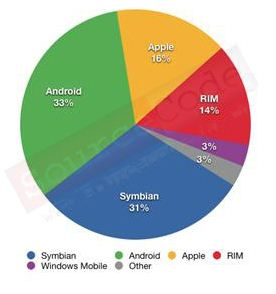
\includegraphics[width=0.5\columnwidth]{Figures/2/maketshare}
		\caption{ส่วนแบ่งการตลาดระบบปฏิบัติการบนสมาร์ทโฟน}{ที่มา :  https://beerkung.wordpress.com/ระบบปฏิบัติการรุ่นล่าส/ระบบปฏิบัติการ-android.html}
		\label{Fig:maketshare}
	\end{figure}

	\subsection{ประวัติความเป็นมาของระบบปฏิบัติการแอนดรอยด์}
	เริ่มต้นระบบปฏิบัติการแอนดรอยด์ถูกพัฒนามาจากบริษัทแอนดรอยด์ (Android Inc.) เมื่อปี พ.ศ 2546 โดยมีนาย แอนดี้ รูบิน (Andy Rubin) ผู้ให้กำเนิดระบบปฏิบัติการนี้และถูกบริษัทกูเกิ้ลเข้าซื้อกิจการเมื่อ เดือนสิงหาคม ปี พ.ศ 2548 โดยบริษัทแอนดรอยด์ ได้กลายมาเป็นบริษัทลูกของบริษัทกูเกิ้ล
	
	ระบบปฏิบัติการแอนดรอยด์ เป็นระบบปฏิบัติการที่พัฒนามาจากการนำเอาแกนกลางของระบบปฏิบัติการลินุกซ์ (Linux Kernel) ซึ่งเป็นระบบปฏิบัติการที่ออกแบบมาเพื่อทำงานเป็นเครื่องให้บริการ (Server) มาพัฒนาต่อ เพื่อให้กลายเป็นระบบปฏิบัติการบนอุปกรณ์พกพา (Mobile Operating System)
	
	ต่อมาเมื่อเดือน พฤศจิกายน ปี พ.ศ 2550 บริษัทกูเกิ้ล ได้ทำการก่อตั้งสมาคม OHA (Open Handset Alliance) เพื่อเป็นหน่วยงานกลางในการกำหนดมาตรฐานกลาง ของอุปกรณ์พกพาและระบบปฏิบัติการแอนดรอยด์ โดยมีสมาชิกในช่วงก่อนตั้งจำนวน 34 รายเข้าร่วม ซึ่งประกอบไปด้วยบริษัทชั้นนำที่ดำเนินธุรกิจด้าการสื่อสาร เช่น โรงงานผลิตอุปกรณ์พกพา บริษัทพัฒนาโปรแกรม ผู้ให้บริการสื่อสาร และผู้ผลิตอะไหล่อุปกรณ์ด้านสื่อสาร   \cite{openhandsetalliance}
	
	หลังจากนั้น เมื่อเดือนตุลาคม ปี พ.ศ 2551 บริษัท กูเกิ้ล ได้เปิดตัวมือถือตัวแรกที่ใช้ระบบปฏิบัติการแอนดรอยด์ ที่ชื่อ T-Mobile G1 หรืออีกชื่อนึงคือ HTC Dream โดยใช้แอนดรอยด์รุ่น 1.1 และหลังจากนั้น ได้มีการปรับพัฒนาระบบปฏิบัติการเป็นรุ่นใหม่ มาเป็นลำดับ
	
	ช่วงต่อมาได้มีการออกผลิตภัณฑ์จากบริษัทต่าง ๆ ออกมาหลากหลายรุ่น หลากหลายยี่ห้อ ตามการพัฒนาระบบปฏิบัติการแอนดรอยด์ ที่มีอยู่อย่างต่อเนื่อง ทำให้สินค้าของแอนดรอยด์ มีให้เลือกอยู่อย่างมากมาย
	
	\subsection{โครงสร้างของระบบปฏิบัติการแอนดรอยด์}
	การทำความเข้าใจโครงสร้างของระบบปฏิบัติการแอนดรอยด์ \cite{androidbook1} ถือว่าเป็นสิ่งสำคัญเพราะถ้านักพัฒนาโปรแกรม สามารถมองภาพโดยรวมของระบบได้ทั้งหมด จะสามารถเข้าใจถึงกระบวนการทำงานได้ดียิ่งขึ้น และสามารถนำไปช่วยในการออกแบบโปรแกรมที่ต้องการพัฒนาเพื่อให้เกิดประสิทธิภาพในการทำงาน
	
	\begin{figure}[H]
		\centering
		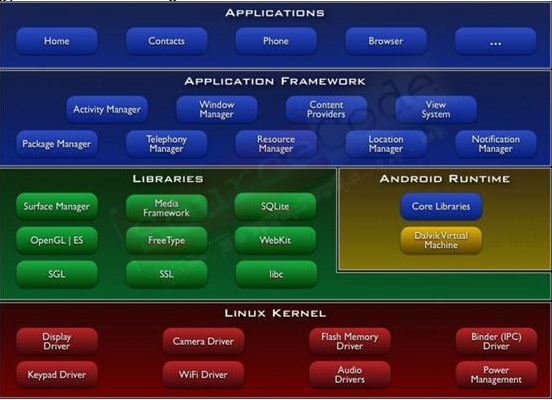
\includegraphics[width=0.8\columnwidth]{Figures/2/androidarchitecture}
		\caption{โครงสร้างของระบบปฏิบัติการแอนดรอยด์}{ที่มา : https://www.theandroid-mania.com/android-architecture/}
		\label{Fig:androidarchitecture}
	\end{figure}
	จากโครงสร้างของระบบปฏิบัติการแอนดรอยด์ในรูปที่ \ref{Fig:androidarchitecture} จะสังเกตได้ว่า มีการแบ่งออกเป็นส่วน ๆ ที่มีความเกี่ยวเนื่องกัน โดยส่วนบนสุดเป็นส่วนที่ผู้ใช้งานทำการติดต่อโดยตรงซึ่งคือส่วนของ Applications ลำดับถัดมาเป็นองค์ประกอบอื่น ๆ ตามลำดับ และสุดท้ายเป็นส่วนที่ติดต่อกับอุปกรณ์โดยผ่านทาง Linux Kernel โครงสร้างของแอนดรอยด์สามารถอธิบายได้ดังนี้

	\begin{enumerate}
		\item Applications ส่วนแอปพลิเคชันหรือส่วนของโปรแกรมที่มากับระบบปฏิบัติการ หรือเป็นกลุ่มของโปรแกรมที่ผู้ใช้งานได้ทำการติดตั้งไว้ โดยผู้ใช้งานสามารถเรียกใช้โปรแกรมต่าง ๆ ได้โดยตรงซึ่งการทำงานของแต่ละโปรแกรมจะเป็นไปตามที่ผู้พัฒนาโปรแกรมได้ออกแบบและเขียนโค้ด (Code) โปรแกรมเอาไว้
		\item Application Framework  เป็นส่วนที่มีการพัฒนาขึ้นเพื่อให้นักพัฒนาสามารถพัฒนาโปรแกรมได้สะดวก และมีประสิทธิภาพมากยิ่งขึ้น โดยนักพัฒนาไม่จำเป็นต้องพัฒนาในส่วนที่มีความยุ่งยากมากๆ เพียงแค่ทำการศึกษาถึงวิธีการเรียกใช้งาน Application Framework ในส่วนที่ต้องการใช้งานแล้วนำมาใช้งาน ซึ่งมีหลายกลุ่มด้วยกัน ตัวอย่างเช่น
			\begin{itemize}
				\item Activities Manager เป็นกลุ่มของชุดคำสั่งที่จัดการเกี่ยวกับวงจรการทำงานของหน้าต่างโปรแกรม (Activity)
				\item Content Providers เป็นกลุ่มของชุดคำสั่ง ที่ใช้ในการเข้าถึงข้อมูลของโปรแกรมอื่น และสามารถแบ่งปันข้อมูลให้โปรแกรมอื่นเข้าถึงได้
				\item View System เป็นกลุ่มของชุดคำสั่งที่เกี่ยวกับการจัดการโครงสร้างของหน้าจอที่แสดงผลในส่วนที่ติดต่อกับผู้ใช้งาน (User Interface)
				\item Telephony Manager เป็นกลุ่มของชุดคำสั่งที่ใช้ในการเข้าถึงข้อมูลด้านโทรศัพท์ เช่น หมายเลขโทรศัพท์ เป็นต้น
				\item Resource Manager เป็นกลุ่มของชุดคำสั่งในการเข้าถึงข้อมูลที่เป็นข้อความและรูปภาพ
				\item Location Manager เป็นกลุ่มของชุดคำสั่งที่เกี่ยวกับตำแหน่งทางภูมิศาสตร์ที่ระบบปฏิบัติการได้รับค่าจากอุปกรณ์
				\item Notification Manager เป็นกลุ่มของชุดคำสั่งที่จะถูกเรียกใช้เมื่อโปรแกรมต้องการแสดงผลให้กับผู้ใช้งาน ผ่านทางแถบสถานะ (Status Bar) ของหน้าจอ
			\end{itemize}
		\item Libraries เป็นส่วนของชุดคำสั่งที่พัฒนาด้วย C/C++ โดยแบ่งชุดคำสั่งออกเป็นกลุ่มตามวัตถุประสงค์ของการใช้งาน เช่น Surface Manage จัดการเกี่ยวกับการแสดงผล Media Framework จัดการเกี่ยวกับการการแสดงภาพและเสียง Open GL|ES และ SGL จัดการเกี่ยวกับภาพ 3 มิติ และ 2 มิติ SQLlite จัดการเกี่ยวกับระบบฐานข้อมูล เป็นต้น
		\item Android Runtime จะมี Darvik Virtual Machine ที่ถูกออกแบบมาเพื่อให้ทำงานบนอุปกรณ์ที่มีหน่วยความจำ (Memmory) หน่วยประมวลผลกลาง (CPU) และพลังงาน (Battery) ที่จำกัดซึ่งการทำงานของ Darvik Virtual Machine จะทำการแปลงไฟล์ที่ต้องการทำงานไปเป็นไฟล์ .DEX ก่อนการทำงานเหตุผลเพื่อให้มีประสิทธิภาพเพิ่มขึ้นเมื่อใช้งานกับหน่วยประมวลผลกลางที่มีความเร็วไม่มากส่วนต่อมาคือ Core Libraries ที่เป็นส่วนรวบรวมคำสั่งและชุดคำสั่งสำคัญโดยถูกเขียนด้วยภาษาจาวา (Java Language)
		\item Linux Kernel เป็นส่วนที่ทำหน้าที่หัวใจสำคัญในจัดการกับบริการหลักของระบบปฏิบัติการ เช่น เรื่องหน่วยความจำ พลังงาน ติดต่อกับอุปกรณ์ต่างๆ ความปลอดภัย เครือข่าย โดยแอนดรอยด์ได้นำเอาส่วนนี้มาจากระบบปฏิบัติการลินุกซ์ รุ่น 2.6 (Linux 26. Kernel) ซึ่งได้มีการออกแบบมาเป็นอย่างดี
	\end{enumerate}
%	\subsection{ข้อเด่นของระบบปฏิบัติการแอนดรอยด์}
%	เนื่องจากระบบปฏิบัติการแอนดรอยด์มีการเจริญเติบโตอย่างรวดเร็วและมีส่วนแบ่งตลาดของอุปกรณ์ด้านนี้ขึ้นทุกขณะ ทำให้กลุ่มผู้ใช้งานและกลุ่มนักพัฒนาโปรแกรมให้ความสำคัญกับระบบปฏิบัติการแอนดรอยด์เพิ่มมากขึ้น
%	
%	เมื่อมองในด้านของกลุ่มผลิตภัณฑ์บริษัทที่มีการพัฒนาผลิตภัณฑ์รุ่นใหม่ ได้มีการนำเอาระบบปฏิบัติการแอนดรอยด์ไปใช้ในสินค้าของตนเองพร้อมทั้งยังมีการปรับแต่งให้ระบบปฏิบัติการมีความสามารถ การจัดวาง โปรแกรมและลูกเล่นใหม่ ๆ ที่แตกต่างจากคู่แข่งในท้องตลาดโดยเฉพาะอย่างยิ่งกลุ่มสินค้าที่เป็นมือถือรุ่นใหม่(SmartPhone)และอุปกรณ์จอสัมผัส(Touch Screen)โดยมีลักษณะแตกต่างกันไป เช่น ขนาดหน้าจอ ระบบโทรศัพท์ ความเร็วของหน่วยประมวลผล ปริมาณหน่วยความจำ แม้กระทั่งอุปกรณ์ตรวจจับ(Sensor)ต่าง ๆ 
%	
%	หากมองในด้านของการพัฒนาโปรแกรม ทางบริษัท Google ได้มีการพัฒนา Application Framework ไว้สำหรับนักพัฒนาใช้งานได้อย่างสะดวกและไม่เกิดปัญหาเมื่อนำชุดโปรแกรมที่พัฒนาขึ้นมา ไปใช้กับอุปกรณ์ที่มีลักษณะต่างกัน เช่น ขนาดจออุปกรณ์ไม่เท่ากัน ก็ยังสามารถใช้งานโปรแกรมได้เหมือนกัน เป็นต้น
	
	\subsection{การจัดการเกี่ยวกับวัฏจักรแอคทิวิตี้ของแอปพลิเคชัน}
	
	ขณะที่ผู้ใช้เปิดใช้งานแอปพลิเคชัน -> ออกจากแอปพลิเคชัน -> แล้วก็กลับเข้ามาในแอปพลิเคชันอีกครั้งแอคทิวิตี้จะมีการย้าย Method ต่างๆ เกิดขึ้นในวัฏจักรแอคทิวิตี้ ยกตัวอย่างเช่น 
	เมื่อแอคทิวิตี้เริ่มทำงานครั้งแรกจะแสดงขึ้นมาอยู่ด้านบนสุดของระบบ (Foreground) และรอรับการทำงานจากผู้ใช้ในระหว่างกระบวนการนี้ระบบจะมีการเรียกใช้งาน Callback Method หรือ Method ที่ถูกเรียกใช้งานอัตโนมัติในแอคทิวิตี้ที่ได้กำหนดการทำงานให้กับ UI และสวนติดต่ออื่น ๆ ไว้ ถ้าผู้ใช้มีการใช้งานใด ๆ ที่เป็นการเรียกแอคทิวิตี้อื่นขึ้นมาหรือสลับไปใช้งานแอปพลิเคชันอื่นระบบจะเรียก Callback Method อีกอันขึ้นมา เช่น ซ่อนแอปพลิเคชันไว้ด้านหลัง Background (ไม่แสดงแอคทิวิตี้แต่ Instance และ Method นั้นยังทำงานอยู่)
	
	ภายใน Callback Method สามารถกำหนดการทำงานในแอคทิวิตี้เมื่อผู้ใช้ออกจากแอปพลิเคชันและกลับเข้ามาใช้งานแอปพลิเคชันใหม่อีกครั้งได้ ตัวอย่าง ถ้าแอปพลิเคชันเป็นแอปพลิเคชัน Streaming Video
	อาจจะสั่งให้ทำการหยุด Video ชั่วคราว และปิดการเชื่อมต่อ Network ไว้ก่อนเมื่อผู้ใช้สลับไปใช้แอปพลิเคชันอื่น
	และทันทีที่ผู้ใช้กลับมาใช้งานแอปพลิเคชันต่อ ก็ให้ทำการเชื่อมต่อกับ Network และก็อนุญาตให้ผู้ใช้กลับไปเล่น Video
	ในตำแหน่งที่ค้างต่อไปทันทีได้โดยที่ไม่ต้องเริ่มต้นแอปพลิเคชันใหม่ เป็นต้น
	
	\subsection{กระบวนการเริ่มทำงานของแอคทิวิตี้ (Activity)}
	ในระบบแอนดรอย์การกำหนดโค้ดเริ่มต้นไว้ในแอคทิวิตี้โดยสัมพันธ์กับ Method ที่ถูกเรียกใช้งานอัตโนมัติ (Callback Method) อย่างเป็นลำดับ ตั้งแต่เริ่มต้นแอคทิวิตี้ไปจนถึงสิ้นสุดและปิดการทำงานของ Activity ลง
	
	\subsection{ทำความรู้จักกับ Lifecycle Callback}
	ในขณะที่แอคทิวิตี้ \cite{ActivityLifeCycle} ทำงานระบบจะเรียกใช้ Callback Method ตามลำดับในลักษณะที่คล้ายกับการก่อพีระมิด นั่นคือ แต่ละขั้นตอนวัฏจักรของแอคทิวิตี้คือส่วนแยกย่อยแต่ละขั้นของพีระมิด
	เช่น เมื่อระบบสร้าง Instance ของแอคทิวิตี้ขึ้นมาใหม่ Method ที่เรียกใช้งานอัตโนมัติ (Callback Method) จะขยับ Activity Method ขึ้นมาด้านบนโดยด้านบนของพีระมิดคือจุดที่แอคทิวิตี้กำลังทำงานแสดงอยู่ด้านหน้า (Foreground Activity) สุดและผู้ใช้กำลังใช้งานอยู่และเมื่อผู้ใช้กำลังจะออกจากแอคทิวิตี้ระบบจะเรียกใช้ Method อื่นซึ่งทำให้ Activity Method
	ถอยกลับไปอยู่ด้านล่างของพีระมิดตามลำดับเพื่อหยุดการทำงานและลบแอคทิวิตี้ออกไป ในบางกรณีแอคทิวิตี้จะย้ายลงมาอยู่บางจุดและรอจังหวะที่จะถูกเรียกกลับขึ้นมาด้านบนอีก เช่น ในกรณีเมื่อผู้ใช้สลับไปใช้งานแอปพลิเคชันอื่นแล้วกลับมาใช้งานอีกครั้ง
	\begin{figure}[H]
		\centering
		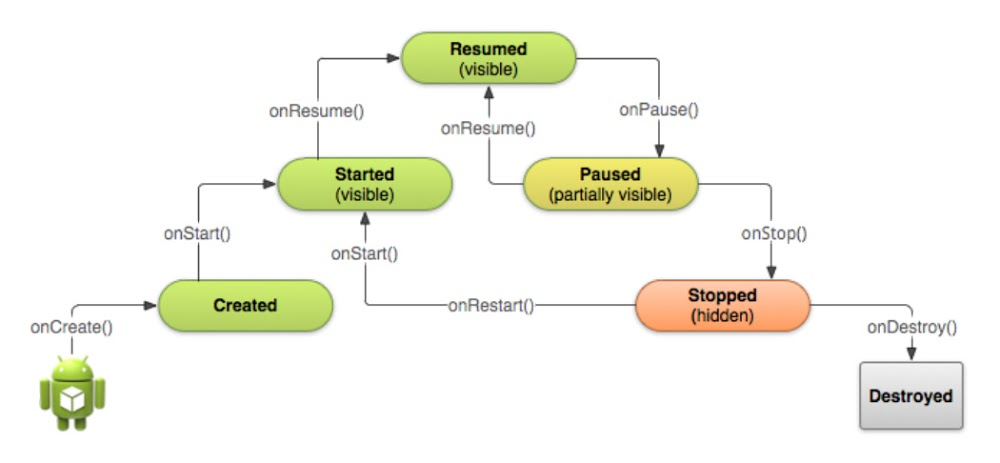
\includegraphics[width=0.8\columnwidth]{Figures/2/lifecycle}
		\caption{วัฏจักรของแอคทิวิตี้บนระบบปฏิบัติการแอนดรอยด์}{ที่มา : https://www.dev2qa.com/android-activity-lifecycle-example/}
		\label{Fig:lifecycle}
	\end{figure}
	จากรูปที่ \ref{Fig:lifecycle} แสดงวัฏจักรของแอคทิวิตี้ในรูปแบบโครงสร้างพีระมิดโดยแสดงให้เห็นว่า Method ที่เรียกใช้
	งานอัตโมัติ (Callback Method) ได้แก่ onCreate(), onStart(), onResume() และ onRestart() จะขยับแอคทิวิตี้ขึ้นไปด้านบนสุดที่ Resumed Method
	และมี Method ได้แก่ onPause(), onStop() และ onDestroy() ที่จะขยับแอคทิวิตี้ลงมาด้านล่าง แอคทิวิตี้ยังสามารถกลับไปทำงานที่ตำแหน่ง Resumed Method จากตำแหน่ง Paused และ Stopped ได้อีกด้วย
	
	ในบางครั้งไม่จำเป็นต้องเรียกใช้งาน Callback Method ทั้งหมดเสมอไปขึ้นกับความซับซ้อนของแอคทิวิตี้ อย่างไรก็ตามเป็นสิ่งสำคัญที่นักพัฒนาควรทำความเข้าใจแต่ละ Method เพื่อให้มั่นใจได้ว่าแอปพลิเคชันของที่ได้พัฒนาตอบสนองเป็นไปตามที่ผู้ใช้คาดหวัง ดังนั้น ในการใช้งาน Callback Method
	ที่ถูกวิธีก็จะช่วยให้แอปพลิเคชันทำงานได้เป็นอย่างดี ดังนี้
	\begin{itemize}
		\item ไม่หยุดการทำงานหรือค้าง กรณีมีสายโทรเข้าหรือมีการสลับไปใช้งานแอปพลิเคชันอื่น 
		\item ไม่ใช้ทรัพยากรที่มีค่าของระบบอย่างสูญเปล่า ถ้าไม่มีการใช้งานแอคทิวิตี้ใดๆ 
		\item ไม่กระทบต่อกระบวนการในขั้นตอนการใช้งานของผู้ใช้กรณีออกจากแอปพลิเคชันแล้วกลับเข้ามาใช้งานอีกครั้ง 
		\item ไม่หยุดการทำงานหรือระบบค้างที่กระทบการใช้งานของผู้ใช้กรณีมีการหมุนหน้าจอแนวนอนและแนวตั้งสลับกัน
	\end{itemize}
	
	เหตุการณ์ที่แอคทิวิตี้มีการเปลี่ยน Method ต่าง ๆ ตามแสดงในรูปที่  \ref{Fig:lifecycle}
	แต่มีอยู่ 3 Method เท่านั้นที่แอคทิวิตี้จะยังคงอยู่คงที่ในช่วงเวลาระยะเวลาหนึ่งไม่เปลี่ยนไป Method อื่นในทันที ได้แก่
		\begin{itemize}
		\item Resumed (แสดงอยู่ ทำงานอยู่) ใน Method นี้แอคทิวิตี้จะแสดงอยู่ด้านหน้าสุดและผู้ใช้กำลังใช้งานอยู่ บ่อยครั้งจะเรียกว่า Running Method
		\item Paused (แสดงหน้าจอบางส่วน ไม่ถูกบังสนิท) ใน Method นี้แอคทิวิตี้จะถูกบดบังด้วยแอคทิวิตี้อื่น เช่น แอคทิวิตี้อื่นที่อยู่ด้านหน้าสุดที่แสดงในลักษณะกึ่งโปรงใสหรือไม่ได้แสดงแบบเต็มหน้าจอ  แอคทิวิตี้ในสถานะนี้จะไม่สามารถรับค่าจากผู้ใช้และทำงานคำสั่งใด ๆ ได้
		\item Stopped (แสดงหน้าจอแบบ Background ผู้ใช้มองไม่เห็น) ใน Method นี้ แอคทิวิตี้จะถูกบดบังอย่างสมบูรณ์และผู้ใช้มองไม่เห็นโดยจะถูกย้ายไปอยู่ด้านหลังในขณะที่อยู่ใน Method นี้
		ค่า Activity Instance และตัวแปรทั้งหมดจะยังคงอยู่แต่จะไม่สามารถถูกเรียกมาใช้งานจากโค้ดใด ๆ ได้
		\end{itemize}
		ในขณะที่ Method อื่น เช่น Created และ Started จะแสดงชั่วคราวแล้วระบบก็จะเปลี่ยนไป Method อื่นในทันทีที่ Method ถูกเรียกใช้งานอัตโนมัติ นั่นคือ หลังจากที่ระบบเรียกใช้งาน onCreate() แล้วก็จะเรียกใช้งาน onStart()
		ทันทีและสุดท้ายตามด้วย onResumne()  ซึ่งก็จะเข้าสู่ Resumed Method ทั้งหมดก็คือวัฏจักรแอคทิวิตี้เบื้อต้น
		
	\subsection{การกำหนด Launcher Activity ในแอปพลิเคชัน}
	เมื่อผู้ใช้กดที่ Icon App จากหน้า Home Screen เพื่อใช้งาน ระบบก็จะเรียก onCreate() Method
	ขึ้นมาทำงานอัตโนมัติเพื่อที่จะเปิดใช้งานแอคทิวิตี้ที่ได้กำหนดให้เป็นแอคทิวิตี้หลัก ("launcher" หรือ "main" ) 
	ซึ่งก็จะเป็นแอคทิวิตี้ที่เป็นหน้าหลักที่ผู้ใช้จะเห็นเมื่อเข้ามาใช้งานแอปพลิเคชัน สามารถกำหนดได้ว่าแอคทิวิตี้ใดที่จะใช้เป็น Activity หลักโดยกำหนดค่าในไฟล์ AndroidManifest.xml
	
	แอคทิวิตี้หลักจะต้องกำหนด ค่าใน manifest ด้วย <intent-filter> 
		\begin{figure}[H]
			{\setstretch{1.0}\begin{lstlisting}
<intent-filter>
<action android:name="android.intent.action.MAIN" />
<category android:name="android.intent.category.LAUNCHER" />
</intent-filter>
					\end{lstlisting}}
					\caption{การกำหนด Launcher Activity ในแอปพลิเคชัน}
					\label{Fig:Launcher}
		\end{figure}
โดยประกอบไปด้วย MAIN action และ LAUNCHER category ดังตัวอย่างดังนี้
				\begin{figure}[H]
					{\setstretch{1.0}\begin{lstlisting}
<Activity android:name=".MainActivity" android:label="@string/app_name">
<intent-filter>
<action android:name="android.intent.action.MAIN" />
<category android:name="android.intent.category.LAUNCHER" />
</intent-filter>
</Activity>
						\end{lstlisting}}
					\caption{การกำหนด Launcher Activity ในแอปพลิเคชัน}
					\label{Fig:category}
				\end{figure}
   ใน Android Studio เมื่อสร้างโปรเจค (Project) ขึ้นมาจะมีการประกาศค่าและกำหนดให้มีการเรียกใช้งาน filter ในไฟล์ AndroidManifest.xml มาให้เรียบร้อยแล้ว ถ้าไม่ได้กำหนด MAIN action และ LAUNCHER category แล้ว App Icon ของจะไม่แสดงในหน้าหลักของลิสรายการแอปพลิเคชันบนหน้าจอสมาร์ทโฟนของผู้ใช้
	\subsection{การสร้าง Instance ใหม่}
	แอปพลิเคชันส่วนใหญ่จะประกอบไปด้วยแอคทิวิตี้หลายอันทำงานแตกต่างกันไป  ไม่ว่าจะเป็นแอคทิวิตี้หลักที่ถูกสร้างขึ้นเมื่อผู้ใช้คลิกที่ icon app หรือแอคทิวิตี้ต่าง ๆ ที่ถูกเรียกใช้งานโดยผู้ใช้ ทั้งหมดล้วนแล้วเป็นสิ่งที่ระบบสร้าง instance ใหม่ของแอคทิวิตี้โดยการเรียกใช้ผ่าน onCreate() Method ต้องใช้ onCreate() Method ในเหตุผลเพื่อเริ่มต้นแอปพลิเคชันซึ่งควรจะเกิดขึ้นเพียงครั้งเดียวตลอดหนึ่งวัฏจักรของแอคทิวิตี้เช่น ใช้ onCreate() กำหนดหน้าตาของแอปพลิเคชันหรือประกาศตัวแปรที่จะถูกใช้งานในคลาส (Class) เป็นต้น ตัวอย่างการใช้งาน onCreate() Method ตามตัวอย่างรูปที่ \ref{Fig:onCreate} แสดง code เพื่อให้เห็นการตั้งค่าเบื่องต้นเช่น การกำหนด User interface(โดยใช้ XML layout ไฟล์) การประกาศตัวแปรต่าง ๆ การตั้งค่ากำหนดเงื่อนไข UI 
					\begin{figure}[H]
						{\setstretch{1.0}\begin{lstlisting}
TextView mTextView; // การประกาศตัวแปรจำหรับ text view ใน layout

@Override
public void onCreate(Bundle savedInstanceMethod) {
	super.onCreate(savedInstanceMethod);

// การกำหนด user interface (โดยใช้ XML layout ไฟล์) 
// ไฟล์ layout ใน project จะอยู่ที่  res/layout/main_Activity.xml 
	setContentView(R.layout.main_Activity);

// กำหนดค่าให้กับ TextView ดังนั้นสามารถเรียกใช้งานผ่านชื่อตัวแปรได้ภายหลัง
	mTextView = (TextView) findViewById(R.id.text_message);

// ตั้งค่าสำหรับกำหนดเงื่อนไข UI 
// ตรวจสอบเพื่อยืนยันว่ากำลังใช้งานบน android  Honeycomb   
// หรือสูงกว่า เพื่อเรียกใช้ ActionBar API  
	if (Build.VERSION.SDK_INT >= Build.VERSION_CODES.HONEYCOMB) {
		// กำหนดให้ icon ใน action bar ไม่ทำงานคล้ายปุ่ม Home  
		ActionBar actionBar = getActionBar();
		actionBar.setHomeButtonEnabled(false);
	}
}
							\end{lstlisting}}
						\caption{การใช้งาน onCreate()}
						\label{Fig:onCreate}
					\end{figure}
		เมื่อ onCreate() ทำงานเสร็จระบบจะเรียก onStart() และ onResume() memthod มาทำงานต่อในทันที แอคทิวิตี้จะไม่อยู่ใน Created Method หรือ Started Method ในทางเทคนิคแอคทิวิตี้จะแสดงขึ้นมาทันทีที่ onStart() ถูกเรียกใช้งานแต่ onResume() จะแสดงตามมาติด ๆ ในทันทีและจะอยู่ใน Resumed Method จนกว่าจะมีการเปลี่ยนแปลงบางอย่างเกิดขึ้นเช่น มีสายโทรเข้าหรือผู้ใช้เปิดไปแอคทิวิตี้อื่นหรือปิดหน้าจอลง
		
		 โครงสร้างของวัฏจักรแอคทิวิตี้ที่เน้นไปที่ 3 Method หลักที่ระบบเรียกใช้อัตโนมัติตามลำดับ เมื่อมีการสร้าง Instance
		 ของแอคทิวิตี้ขึ้นมาใหม่ ได้แก่ onCreate(), onStart() และ onResume() เมื่อลำดับการทำงานเสร็จสิ้นลงแอคทิวิตี้จะ
		 มาอยู่ที่ Resumed Method ซึ่งผู้ใช้ใช้งานอยู่จนกว่าจะเปลี่ยนไปเรียกใช้งานแอคทิวิตี้อื่นขึ้นมา
		 
	\subsection{การสิ้นสุดการทำงานของแอคทิวิตี้ (Destroy Activity)}
	ในขณะที่วัฏจักรของแอคทิวิตี้มี Method แรกคือ onCreate() และ Method สุดท้ายคือ onDestroy()
	ระบบจะเรียก Method นี้ในแอคทิวิตี้เป็นสัญญาณว่า Activity instance นี้จะถูกลบบออกอย่างสมบูรณ์จากหน่วยความจำของระบบ (System memory)
	
	แอปพลิเคชันส่วนใหญ่ไม่จำเป็นต้องกำหนด Method นี้เพราะ local class ถูกทำลายไปพร้อมกับแอคทิวิตี้และแทบจะถูกลบไปอย่างสมบูร์ในระหว่างเรียกใช้งาน onPause() และ onStop() อย่างไรก็ตามถ้าแอคทิวิตี้ของมีการกำหนดให้มีการทำงานแบบ background (ทำงานอยู่เบื้องหลัง) ในขั้นตอน onCreate() ด้วยแล้วหรือมีการใช้งานทรัพยากรของระบบเป็นระยะเวลานานเป็นเหตุให้ความจำถูกใช้งานจำนวนมาก หากไม่ทำการปิดการใช้งาน จึงควรอย่างยิ่งที่จะเรียกใช้งาน Method onDestroy() เพื่อคืนค่าหน่วยความจำให้ระบบ
						\begin{figure}[H]
							{\setstretch{1.0}\begin{lstlisting}
@Override
public void onDestroy() {
	super.onDestroy();  // เรียกใช้งาน superclass ทุกครั้งเสมอ

// หยุดการติดตามหรือตรวจจับ Method ของ Activity 
	android.os.Debug.stopMethodTracing();
}
								\end{lstlisting}}
							\caption{การใช้งาน onDestroy()}
							\label{Fig:onDestroy}
						\end{figure}
	ระบบจะเรียกใช้งาน onDestroy() หลังจากเรียกใช้งาน onPause() และ onStop() แล้วในทุกเหตุการณ์ ยกเว้นกรณีมีการกำหนดให้เรียกใช้ finish() ภายใน onCreate() Method ในกรณีเช่น Activity หยุดชั่วคราวเพื่อทำการเรียกใช้งานแอคทิวิตี้อื่นข้ามาแล้วทำการกำหนดให้มีการเรียกใช้งาน finish() ที่กำหนดใน onCreate() Method เพื่อทำลายแอคทิวิตี้ในกรณีนี้ระบบจะทำการเรียก onDestroy() ทันทีโดยไม่ผ่าน Callback Method อื่นเช่น ไม่ผ่าน onPause() หรือ onStop() แบบนี้เป็นต้น
	

\section{ความรู้พื้นฐาน Java}
Java \cite{java6} เป็นภาษาเขียนโปรแกรมเพื่อวัตถุประสงค์ทั่วไป โดยสามารถทำงานได้พร้อมกัน เป็นภาษาที่สร้างมาจากคลาส และสนับสนุนการเขียนโปรแกรมแบบออบเจ็คอย่างสมบูรณ์ และถูกออกแบบมาให้พร้อมสำหรับการใช้งานมากที่สุด ซึ่งมีเมธอดและคลาสต่าง ๆ อำนวยความสะดวกให้ใช้มากมาย โดยภาษา Java นั้นมีความตั้งใจว่าจะทำให้นักพัฒนาออกแบบและพัฒนาโปรแกรมน้อยลง นั่นคือการเขียนเพียงครั้งเดียว แต่นำไปใช้งานได้ทุกที่หรือทุกแพลตฟอร์ม

แอปพลิเคชันของภาษา Java นั้นโดยปกติแล้วจะคอมไพล์เป็น bytecode ที่สามารถรันได้ใน Java virtual machine (JVM) ขึ้นกับสถาปัตยกรรมของคอมพิวเตอร์นั้นๆ และใน ปี 2016 ภาษา Java เป็นภาษาที่ได้รับความนิยมและใช้มากที่สุดในโลก โดยเฉพาะการใช้พัฒนาเว็บแอปพลิเคชัน

	\subsection{ประวัติความเป็นมาของภาษา Java}
	James Gosling Mike Sheridan และ Patrick Naughton ได้เริ่มก่อตั้งโปรเจ็คภาษา Java ของพวกเขาเมื่อปี 1991 โดยในตอนแรกมันถูกพัฒนาสำหรับทีวีที่สามารถมีปฎิสัมพันธ์ได้ เช่น เล่นเกมในทีวีได้ แต่มันยากเกินไปในการที่จะใช้งานกับสายเคเบิลของทีวีดิจิตอลในเวลานั้น ในตอนแรกภาษา Java ใช้ชื่อว่า Oak เพราะว่ามีต้นโอ็คยื่นออกไปยังออฟฟิศของ Gosling ต่อมาใช้ชื่อว่า Green และในตอนท้ายใช้ชื่อว่า Java มีที่มาจากกาแฟ Java 
	
	ภาษาได้รับการออกแบบให้มีรูปแบบทางภาษาเหมือนภาษา C และ C++ ซึ่งทำให้โปรแกรมเมอร์ส่วนมากนั้นคุ้นเคยกับมันได้ดีขึ้น และ Sun Microsystems เผยแพร่ Java 1.0 ในปี 1995 โดยมีคำกล่าวว่า "Write Once, Run Anywhere" (WORA) ซึ่งมันฟรี เขียนเพียงครั้งเดียวและสามารถนำไปรันได้บนทุกแพลตฟอร์ม
	
	\subsection{Java Compiler}
	ในการเขียนโปรแกรมในภาษา Java ต้องการ Java Compiler เพื่อทำการแปลงโค้ดของโปรแกรมที่เขียนเป็น bytecode เพื่อนนำไปรันในแต่ละแพลตฟอร์มต่อไป โดยเรียกว่า Java Platform (JDK) ซึ่งประกอบไปด้วยคอมไพล์เลอร์ ในการแปลงโค้ดภาษา Java ให้เป็น Bytecode และ Java virtual machine (JVM) สำหรับรันโปรแกรมของภาษา Java ในแต่ละแพลตฟอร์ม สำหรับในบทเรียนนี้จะใช้ IDE ในการพัฒนาเพื่อความสะดวกและรวดเร็ว
	
	\subsection{โครงสร้างของภาษา Java}

  \begin{figure}[H]
    \begin{minted}[frame=lines,framesep=2mm,baselinestretch=1.15,fontsize=\footnotesize,linenos]{java}
    public class ClassName {
      public static void main(String[] args) {
        System.out.println("Hello สวัสดี");
      }
    }
    \end{minted}
    \caption{ตัวอย่างโปรแกรมภาษา Java ด้วย minted}
    \label{Fig:JavaClassMinted}
  \end{figure}
  
  รูปที่ \ref{Fig:JavaClassMinted} แสดงให้เห็นผลลัพธ์ของการใช้ minted เพื่อแสดงคำสั่งในเอกสาร Latex

	\begin{itemize}
		\item Package เป็นกลุ่มของคลาสหรือไลบรารี่มาตรฐานของภาษา Java ที่มีฟังก์ชันต่าง ๆ ให้ใช้มากมาย
		\item Class ในส่วนของการประกาศคลาส จะต้องประกาศคลาสให้ชื่อตรงกับไฟล์เสมอ นอกจาก Inner คลาสที่อยู่ในคลาสเดียวกัน โดยชื่อคลาสนั้นควรจะขึ้นต้นด้วยตัวใหญ่และถ้ามีหลายคำให้ใช้ตัวพิมพ์ใหญ่แบ่ง ดังตัวอย่างในรูปที่ \ref{Fig:ClassName}
				\begin{figure}[H]
					{\setstretch{1.0}\begin{lstlisting}
public class ClassName {
...
}
						\end{lstlisting}}
					\caption{การงประกาศคลาสในภาษา Java}
					\label{Fig:ClassName}
				\end{figure}
			\item Method หลังจากคลาสสร้างแล้ว จะเป็นประกาศเมธอดภายในคลาส โดยในการที่จะรันโปรแกรมได้จะต้องมีเมธอดที่ชื่อว่า Main ดังตัวอย่างในโปรแกรมด้านบน มันเป็นที่แรกที่โปรแกรมจะเริ่มทำงาน \ref{Fig:ClassName}
			\begin{figure}[H]
				{\setstretch{1.0}\begin{lstlisting}
public static void main (String[] args) {
...
}
					\end{lstlisting}}
				\caption{การงประกาศเมธอด main ในภาษา Java}
				\label{Fig:main}
			\end{figure}
			\item Methodments เป็นคำสั่งของโปรแกรมเพื่อให้โปรแกรมทำงานตามต้องการ เช่น System.out.println("Hello World!"); เป็นการแสดงผลข้อความออกทางหน้าจอ โดยปกติโปรแกรมมักจะมีหลายคำสั่ง
			\item Semicolon ทุกคำสั่งการทำงานของโปรแกรมในภาษา Java จะจบด้วยเครื่องหมาย Semicolon (;) นั่นหมายความว่าสามารถเขียนโปรแกรมแบบไหนก็ได้ โดยคอมไพเลอร์จะทราบอัตโนมัติว่าสิ้นสุดคำสั่งที่ไหน
			\item ในภาษา Java สามารถใช้ White space ได้อย่างอิสระตามที่ต้องการ โดย White space จะประกอบไปด้วย Space bar Tab และ Enter (return) เพราะว่าคอมไพเลอร์ตรวจการสิ้นสุดของคำสั่งด้วย ; ใช้ while space ทำให้โค้ดอ่านเข้าใจง่าย และเป็นระเบียบ
			\item Literals คือค่าของข้อมูลใดๆ ที่กำหนดให้กับตัวแปรได้ เรียกว่า Constant Literals ทุกค่าที่เป็นไปได้ เช่น "MarcusCode" เป็น String Literals 10 เป็น Integer Literals หรือ true เป็น Boolean Literals โดย Literals เป็นได้แค่ Primitive data type เท่านั้น ตัวอย่างการกำหนดค่าหรือ Literals ให้กับตัวแปร
			\item Expression เป็นการกระทำระหว่างตัวแปรกับตัวดำเนินการเพื่อให้ได้ผลลัพธ์ใหม่ เช่น 4 + 3 เป็น expression ของการบวกเลขและได้ได้ผลลัพธ์เท่ากับ 7 หรือ 1 == 1 เป็น expression ของการเปรียบเทียบระหว่างค่าสองค่าว่าเท่ากันหรือไม่ และได้ผลลัพธืเป็น true
			\item Keyword คือคำที่สงวนไว้ในภาษา Java นั่นหมายความว่าไม่สามารถนำคำเหล่านี้ไปประกาศเป็นชื่อตัวแปร เมธอด หรือว่าคลาสได้ เพราะว่า Keyword ถูกใช้โดยคอมไพเลอร์เพื่อให้มันทำงานได้สมบูรณ์
		\end{itemize}
	
	\section{ความรู้พื้นฐาน Java Script}
	 JavaScript \cite{js} คือ ภาษาคอมพิวเตอร์สำหรับการเขียนโปรแกรมบนระบบอินเทอร์เน็ต ที่กำลังได้รับความนิยมอย่างสูง Java JavaScript เป็นภาษาสคริปต์เชิงวัตถุที่เรียกว่า "สคริปต์"  (Script) ซึ่งในการสร้างและพัฒนาเว็บไซต์ (ใช่ร่วมกับ HTML) เพื่อให้เว็บไซต์ของดูมีการเคลื่อนไหว สามารถตอบสนองผู้ใช้งานได้มากขึ้น ซึ่งมีวิธีการทำงานในลักษณะ "แปลความและดำเนินงานไปทีละคำสั่ง" (Interpret) หรือเรียกว่า อ็อบเจ็กโอเรียนเต็ด (Object Oriented Programming) ที่มีเป้าหมายในการออกแบบและพัฒนาโปรแกรมในระบบอินเทอร์เน็ตสำหรับผู้เขียนด้วยภาษา HTML สามารถทำงานข้ามแพลตฟอร์มได้ โดยทำงานร่วมกับภาษา HTML และภาษา Java Script ทำงานได้ทั้งทางฝั่งไคลเอนต์ (Client) และทางฝั่งเซิร์ฟเวอร์ (Server) 
	 
	 JavaScript ถูกพัฒนาขึ้นโดย เน็ตสเคปคอมมิวนิเคชันส์ (Netscape Communications Corporation) โดยใช้ชื่อว่า Live Script ออกมาพร้อมกับ Netscape Navigator2.0 เพื่อใช้สร้างเว็บเพจโดยติดต่อกับเซิร์ฟเวอร์แบบ Live Wire ต่อมาเน็ตสเคปจึงได้ร่วมมือกับ บริษัทซันไมโครซิสเต็มส์ปรับปรุงระบบของบราวเซอร์เพื่อให้สามารถติดต่อใช้งานกับภาษาจาวาได้ และได้ปรับปรุง LiveScript ใหม่เมื่อ ปี 2538 แล้วตั้งชื่อใหม่ว่า JavaScript 
	 
	 JavaScript สามารถทำให้ การสร้างเว็บเพจ มีลูกเล่น ต่าง ๆ มากมายและสามารถโต้ตอบกับผู้ใช้ได้อย่างทันที เช่น การใช้เมาส์คลิกหรือการกรอกข้อความในฟอร์ม เป็นต้น 
	 
	 เนื่องจาก JavaScript ช่วยให้ผู้พัฒนาสามารถสร้างเว็บเพจได้ตรงกับความต้องการและมีความน่าสนใจมากขึ้นประกอบกับเป็นภาษาเปิด ที่ใครก็สามารถนำไปใช้ได้ ดังนั้นจึงได้รับความนิยมเป็นอย่างสูง มีการใช้งานอย่างกว้างขวาง รวมทั้งได้ถูกกำหนดให้เป็นมาตรฐานโดย ECMA การทำงานของ JavaScript จะต้องมีการแปลความคำสั่ง ซึ่งขั้นตอนนี้จะถูกจัดการโดยบราวเซอร์ (เรียกว่าเป็น client-side script) ดังนั้น JavaScript จึงสามารถทำงานได้ เฉพาะบนบราวเซอร์ที่สนับสนุน ซึ่งปัจจุบันบราวเซอร์เกือบทั้งหมดก็สนับสนุน JavaScript แล้ว อย่างไรก็ดีสิ่งที่ต้องระวังคือ JavaScript มีการพัฒนาเป็นเวอร์ชั่นใหม่ ๆ ออกมาด้วยดังนั้น ถ้านำโค้ดของเวอร์ชั่นใหม่ไปรันบนบราวเซอร์รุ่นเก่าที่ยังไม่สนับสนุนอาจจะทำให้เกิดข้อผิดพลาด (Error) ได้
	 
	 \subsection{ลักษณะการทำงานของ JavaScript}
	 JavaScript เป็นภาษาสคริปต์เชิงวัตถุหรือเรียกว่าอ็อบเจ็กโอเรียนเต็ด (Object Oriented Programming) ที่มีเป้าหมายในการออกแบบและพัฒนาโปรแกรมในระบบอินเทอร์เน็ตสำหรับผู้เขียนเอาสารด้วยภาษา HTML สามารถทำงานข้ามแพลตฟอร์มได้ทำงานร่วมกับภาษา HTML และภาษาจาวาได้ทั้งทางฝั่งไคลเอนต์ (Client) และ ทางฝั่งเซิร์ฟเวอร์ (Server) โดยมีลักษณะการทำงานดังนี้ 
	 \begin{itemize}
		 \item Navigator JavaScript เป็น Client-Side JavaScript ซึ่งหมายถึง JavaScript ที่ถูกแปลทางฝั่งไคลเอนต์ หมายถึงฝั่งเครื่องคอมพิวเตอร์ของผู้ใช้ไม่ว่าจะเป็นเครื่องพีซี (Personal computer, PC) เครื่องแมคอินทอช (Macintosh) หรืออื่น ๆ จึงมีความเหมาะสมต่อการใช้งานของผู้ใช้ทั่วไปเป็นส่วนใหญ่ 
		 \item LiveWire JavaScript เป็น Server-Side JavaScript ซึ่งหมายถึง JavaScript ที่ถูกแปลทางฝั่งเซิร์ฟเวอร์ (หมายถึงฝั่งเครื่องคอมพิวเตอร์ของผู้ให้บริการเว็บโดยอาจจะเป็นเครื่องของซันซิลิคอมกราฟิกส์หรืออื่น ๆ) สามารถใช้ได้เฉพาะกับ LIveWire ของเน็ตสเคป โดยตรง
	 \end{itemize}
	
	 \subsection{JavaScript กับ HTML}
	 การเขียน JavaScript อาจเขียนรวมอยู่ในไฟล์เดียวกันกับ HTML ได้ ซึ่งแตกต่างจากการเขียนโปรแกรมภาษา Java ที่ต้อง เขียนแยกออกเป็นไฟล์ต่างหากไม่สามารถเขียนรวมอยู่ในไฟล์เดียวกับ HTML ได้ วิธีการเขียน JavaScript เพื่อสั่งให้เว็ปเพจทำงาน มีอยู่ด้วยกัน 2 วิธี ดังนี้
	 \begin{itemize}
	 	\item เขียนด้วยชุดคำสั่งและฟังก์ชันของ JavaScript เอง
	 	\item เขียนตามเหตการณ์ที่เกิดขึ้นตามการใช้งานจากชุดคำสั่งของ HTML
	 \end{itemize}
	  เมื่อเริ่มใช้งานโปรแกรมบราวเซอร์จะอ่านข้อมูลจากส่วนบนของเพจ HTML และทำงานไปตามลำดับจาก บนลงล่าง (top-down) โดยเริ่มที่ส่วน < HEAD >...< /HEAD > ก่อนจากนั้นจึงทำงานในส่วน < BODY >...< /BODY > เป็นลำดับต่อมา การทำงานของ JavaScript ดูไม่แตกต่างไปจาก HTML เท่าใดนัก แต่ HTML จะวางเลย์เอาต์โครงสร้างของอ็อบเจ็กต์ภายใน และส่วนเชื่อมโยงกับเว็บเพจเท่านั้น ในขณะที่ JavaScript สามารถเพิ่มเติมส่วนของการเขียนโปรแกรมและลอจิกเข้าไป
	 
	 \subsection{โครงสร้างภาษา}
	 	\begin{enumerate}
		 \item ตัวแปร (Variable) หมายถึง ชื่อหรือสัญลักษณ์ที่ตั้งขึ้นสำหรับการเก็บค่าใด ๆ ที่ไม่คงที่ โดยการจองเนื้อที่ในหน่วยความจำของระบบเครื่องที่เก็บข้อมูลซึ่งสามารถอ้างอิงได้ มีขนาดขึ้นอยู่กับชนิดของข้อมูลและค่าของข้อมูล ซึ่งค่าในตัวแปรนี้สามารถเปลี่ยนแปละได้ตามคำสั่งในการประมวลผล
		 
		 \item การตั้งชื่อ (Identifier or Name) เป็นชื่อที่ตั้งขึ้นมาเพื่อกำหนดให้เป็นชื่อของโปรแกรมหลัก, ฟังก์ชัน, ตัวแปร, ค่าคงที่, คำสั่ง และคำสงวน โดยมีหลักการตั้งชื่อว่า
			 \begin{itemize}
				\item ขึ้นต้นด้วยตัวอักษรในภาษาอังกฤษ ตามด้วยตัวอักษรหรือตัวเลขใด ๆ ก็ได้ 
				\item ห้ามเว้นช่องว่าง 
				\item ห้ามใช้สัญลักษณ์พิเศษ ยกเว้นขีดล่าง (\_) และดอลล่าร์ (\$) 
				\item สำหรับความยาวของชื่อใน JavaScript จะมีความยาวเท่าใดก็ได้ แต่ที่นิยมใช้ ไม่เกิน 20 ตัวอักษร 
				\item การตั้งชื่อมีข้อพึงระวังว่า จะต้องไม่ซ้ำกับคำสงวน (Reserve word) และตัวอักษรของชื่อจะจำแนกแตกต่างกันระหว่างอักษรตัวพิมพ์เล็กกับอักษรตัวพิมพ์ใหญ่ 
			    \item ควรจะตั้งชื่อโดยให้ชื่อนั้นมีสื่อความหมายให้เข้ากับข้อมูล สามารถอ่านและเข้าใจได้ 
				ตัวอย่างชื่อที่ถูกต้อง Hahaha, I\_Love\_you, Doll\$ เป็นต้น
			 \end{itemize}
		 \item คำสงวน(Reserve word)เป็นคำที่มีความหมายเฉพาะตัวในภาษา JavaScript สงวนไม่ให้มีการตั้งชื่อซ้ำกับชื่อโปรแกรม, ฟังก์ชัน, ตัวแปร, ค่าคงที่ และคำสั่ง คำสงวน สามารถเรียกใช้ได้ทันทีโดยไม่ต้องมากำหนดความหมายใหม่แต่อย่างใด
	
		 \item ชนิดของข้อมูลของตัวแปร (Data Type) เป็นการกำหนดประเภทค่าของข้อมูลให้กับตัวแปร เพื่อให้เหมาะสมกับการอ้างอิงข้อมูลจากตัวแปรในการใช้งาน ชนิดข้อมูลของตัวแปรนั้นมีอยู่ด้วยกัน 4 ชนิด ได้แก่
			 \begin{itemize}
				 \item number หมายถึง ข้อมูลชนิดตัวเลข ประกอบด้วย เลขจำนวนเต็ม (Integer) และเลขจำนวนจริง (Floating) 
				 \item logical หมายถึง ข้อมูลทางตรรกะ มี 2 สถานะ คือ จริง (True) และเท็จ (False) 
				 \item string หมายถึง ข้อมูลที่เป็นข้อความ ซึ่งจะต้องกำหนดไว้ในเครื่องหมายคำพูด ("...") 
				 \item null หมายถึง ไม่มีค่าข้อมูลใดๆ ซึ่งค่า null ใช้สำหรับการยกเลิกพื้นที่เก็บค่าของตัวแปรออกจากหน่วยความจำ 
			 \end{itemize}
		 \item การประกาศตัวแปร (Declarations) เป็นการกำหนดชื่อและชนิดข้อมูลให้กับตัวแปรเพื่อนำไปใช้ในโปรแกรม โดยการตั้งชื่อจะต้องคำนึงถึงค่าของข้อมูลและ ชนิดของข้อมูลที่อ้างอิง นอกจากนี้การตั้งชื่อควรให้สื่อความหมายของข้อมูล และอักษรของชื่อจะจำแนกแตกต่างกันระหว่างอักษรตัวพิมพ์เล็กกับอักษรตัวพิมพ์ใหญ่
		 
		 รูปแบบ
		 Var ชื่อตัวแปร;
		 เป็นรูปแบบการประกาศตัวแปรปกติหรือ Var ชื่อตัวแปร = ข้อมูล; เป็นรูปแบบการกำหนดค่าเริ่มต้น
		 ในกรณีที่ต้องการกำหนดตัวแปรหลายตัวในบรรทัดเดียวกันให้ใช้เครื่องหมาย คอมม่า ( , ) คั่นระหว่างชื่อตัวแปรและปิดท้ายด้วยเครื่องหมายเซมิโคล่อน ( ; )
		 การกำหนดค่าให้กับตัวแปร
		 
		 รูปแบบ
		 ชื่อตัวแปร = ค่าของข้อมูล
		 โดยที่ค่าของข้อมูล ได้แก่
		 \begin{itemize}
		 	\item ข้อมูลที่เป็นตัวเลข โดยกำหนดตัวเลขไปได้เลย เช่น num = 500
		 	\item ข้อมูลในทางตรรกะ ได้แก่ จริง (True) หรือ เท็จ (False) เช่น test = True; 
		 	\item ข้อมูลสตริง ให้กำหนดอยู่ในเครื่องหมายคำพูด ("...") เช่น name = "Adisak";
		 \end{itemize}
		 ตัวแปรมี 2 จำพวก หากกำหนดชื่อตัวแปรไว้ที่โปรแกรมหลักโดยไม่ได้อยู่ภายในขอบเขตฟังก์ชันใด ๆ เรียกว่าเป็นตัวแปรแบบโกลบัล (Global) ตัวแปรจำพวกนี้จะมีค่าคงอยู่ในหน่วยความจำตลอกการทำงานของโปรแกรม ทำให้สามารถเรียกใช้ได้จากทุก ๆ ส่วนของโปรแกรม รวมถึงภายในฟังก์ชันต่าง ๆ ด้วย
		 แต่ถ้ากำหนดตัวแปรไว้ภายในขอบเขตฟังก์ชันใด ๆ จะเรียกว่าเป็นตัวแปรแบบ โลคัล (Local) เพราะจะเป็นตัวแปรที่มีค่าคงอยู๋ และสามารถเรียกใช้ได้เฉพาะ ภายในขอบเขตของฟังก์ชันนั้น ๆ เท่านั้น 
		 
		 \item ตัวแปรแบบอาร์เรย์ (Array) หมายถึงตัวแปรซึ่งมีค่าได้หลายค่าโดยใช้ชื่ออ้างอิงเพียงชื่อเดียว ด้วยการใช้หมายเลขลำดับเป็นตัวจำแนกความแตกต่างของค่าตังแปรแต่ละตัว ถ้าจะเรียกตัวแปรชนิดนี้ว่า "ตัวแปรชุด" ก็เห็นจะไม่ผิดนัก ตัวแปรชนิดนี้มีประโยชน์มาก ลองคิดถึงค่าข้อมูลจำนวน 100 ค่า ที่ต้องการเก็บไว้ในตัวแปรจำนวน 100 ตัว อาจทำให้ต้องกำหนดตัวแปรที่แตกต่างกันมากถึง 100 ชื่อ กรณีอย่างนี้ควรจะทำอย่างไรดี แต่ด้วยการใช้สมบัติอาร์เรย์ สามารถนำตัวแปรหลาย ๆ ตัวมาอยู่รวมเป็ฯชุดเดียวกันได้และสามารถเรียกใช้ตัวแปรทั้งหมดโดยระบุผ่านชื่อเพียงชื่อเดียวเท่านั้น ด้วยการระบุหมายเลขลำดับ หรือ ดัชนี (index) กำกับตามหลังชื่อตัวแปร ตัวแหรเพียงชื่อเดียวจึงมีความสามารถเทียบได้กับตัวแปรนับร้อยตัว พันตัว (ตัวที่ 1) ในตัวแปรแบบอาร์เรย์มีดัชนีเป็น 0 ส่วนตัวแปรต่อ ๆ ไปก็จะมีดัชนีเป็น 1,2,3,... ไปตามลำดับ เมื่อต้องการระบุชื่อตัวแปรแบบอาร์เรย์แต่ละตัว ก็จะใช้รูปแบบ name[0], name[1],... เรียงต่อกันไปเรื่อย ๆ สามารถสร้างตัวแปรอาร์เรย์ใหม่ด้วย myArray = new Array() ดังนี้
		 			\begin{figure}[H]
		 				{\setstretch{1.0}\begin{lstlisting}
 myArray[0] = 17;
 myArray[1] = "Nun";
 myArray[2] = "Stop";
		 					\end{lstlisting}}
		 				\caption{ตัวแปรอาร์เรย์}
		 				\label{Fig:ตัวแปรอาร์เรย์}
		 			\end{figure}	

		 \item ค่าคงที่ (Literal หรือ Constant) หมายถึง ค่าของข้อมูลที่เมื่อกำหนดแล้วจะทำการเปลี่ยนแปลงค่าเป็นอย่างอื่นไม่ได้ ชนิดข้อมูลของค่าคงที่ได้แก่
			 \begin{itemize}
				  \item เลขจำนวนเต็ม (Integer) เป็นตัวเลขที่ไม่มีเศษทศนิยม สามารถเขียนให้อยู่ในแบบ เลขฐานสิบ (0-9), เลขฐานสิบหก (0-9, A-F) หรือ เลขฐานแปด (0-7) โดยการเขียนเลขฐานแปดให้ นำหน้าด้วย O  (Octenary) ส่วนการเขียนเลขฐานสิบหกให้นำหน้าด้วย Ox หรือ OX (Hexadenary) 
				  \item เลขจำนวนจริง (Floating) ใช้รูปแบบการเขียนโดยประกอบไปด้วยตัวเลข จุดทศนิยมและตัวเลขยกกำลัง E (Exponential) เช่น 
				  ◦ 5.00E2 จะหมายถึงค่า 5.00 คูณด้วย 10 ยกกำลัง 2 จะมีค่าเป็น 500 
				  ◦ 3.141E5 จะหมายถึงค่า 3.141 คูณด้วย 10 ยกกำลัง 5 จะมีค่าเป็น 314,1000 
				  \item ค่าบูลีน (Boolean) เป็นค่าคงที่เชิงตรรกะ คือมีค่าเป็น จริง(True) และ เท็จ(False) เท่านั้น 
				  \item ข้อความสตริง (String) เป็นค่าคงที่แบบข้อความที่อยู่ภายในเครื่องหมายคำพูด ("..." หรือ '...') เช่น "บริษัท เอ็กซ์ทรีม จำกัด", 'นางนฤมล เวชตระกูล' 
			 \end{itemize}
		
		 \item รหัสคำสั่งพิเศษ (Character escape code) เป็นการกำหนดรหัสเพื่อควบคุมงานพิมพ์สตริงโดยใช้เครื่องหมาย Backslash นำหน้าตัวอักษรที่ต้องการกำหนดเป็นรหัส เพื่อให้กลายเป็นรหัสคำสั่งพิเศษ
		 รหัส Character escape code
		 
		 \item นิพจน์ (Expression) เป็นข้อคำสั่งที่ใช้กำหนดค่าของข้อมูล เช่น การบวกตัวเลข การเปรียบเทียบข้อมูล โดยการกำหนดชื่อของตัวแปร ตามด้วยเครื่องหมายที่ต้องการกระทำ (Operations) ต่อข้อมูลเป็นผลให้เกิดค่าข้อมูลใหม่ค่าหนึ่งให้กับตัวแปรเพื่อนำไปใช้งาน
		 
		 นิพจน์ JavaScript มีด้วยกัน 3 ชนิดดังนี้
			 \begin{itemize}
			 	 \item นิพจน์คณิตศาสตร์ (Arithmetic) เป็นนิพจน์ที่ใช้เครื่องหมายทางคณิตศาสตร์เป็นตัวกระทำ ผลลัพธ์ที่ได้จะมีค่าเป็นตัวเลขให้กับตัวแปร
			 	 เช่น ให้ตัวแปร num เก็บตัวเลข 5000 จะเขียนได้ดังนี้
			 	 num = 5000;
			 	 \item นิพจน์ตรรกะ (Logical) เป็นนิพจน์ในการเปรียบเทียบข้อมูลโดยใช้เครื่องหมายในการเปรียบเทียบเพื่อตรวจสอบข้อมูลในการเปรียบเทียบว่าจริงหรือเท็จ
			 	 เช่น กำหนดให้ 
			 	 		 			\begin{figure}[H]
			 	 		 				{\setstretch{1.0}\begin{lstlisting}
a = 50;
b = 70;
c = b>a;
			 	 		 					\end{lstlisting}}
			 	 		 				\caption{การเปรียบเทียบว่าจริงหรือเท็จ}
			 	 		 				\label{Fig:การเปรียบเทียบว่าจริงหรือเท็จ}
			 	 		 			\end{figure}	
			 	 ผลลัพธ์ที่ได้คือ c จะมีค่าเป็นจริง (True)
			 	 \item นิพจน์ข้อความ (String)
			 	 เป็นนิพจน์เกี่ยวกับการกำหนดข้อความ การเชื่อประโยคข้อความ ใช้ประมวลผลข้อความในลักษณะต่าง ผลลัพธ์ที่ได้จึงมีค่าเป็ฯตัวอักษรหรือข้อความเสมอ
			 	 เช่น ให้ตัวแปร name เก็บชื่อ Adisak จะเขียนได้ดังนี้
			 	 name = "Adisak";
			 \end{itemize}
		
		 \item ตัวดำเนินการ (Operator) หมายถึง เครื่องหมายกำหนดกรรมวิธีทางคณิตศาสตร์, พีชคณิต, บูลีน, การเปรียบเทียบ ระหว่างข้อมูล 2 ตัว ซึ่งเรียกว่า โอประแรนด์ (Operand)  โดยอาจมีค่าเป็นตัวเลข ข้อความ ค่าคงที่ หรือตัวแปรต่าง ๆ
		 
		 \item ชนิดของตัวดำเนินการ
			 \begin{itemize}
			 			 \item ตัวดำเนินการคณิตศาสตร์ (Arithmetic operator) หมายถึง ใช้สำหรับคำนวณโอประแรนด์ที่เป็นค่าคงที่หรือตัวแปรก็ได้ โดยให้ค่าผลลัพธ์เป็นตัวเลขค่าเดียว
			 			 
			 			 \item ตัวดำเนินการเชิงเปรียบเทียบ (Comparison operator) หมายถึง เครื่องหมายในการเปรียบเทียบข้อมูล ผลลัพธ์ที่ได้จะมีค่าตรรกบูลลีนเป็น จริง (True) และ เท็จ (False)
			 			 
			 			 \item ตัวดำเนินการเชิงตรรกะ (Logical operator) เป็นเครื่องหมายที่ให้ค่าจริง (True) และ เท็จ (False) ในการเปรียบเทียบ
			 			 
			 			 \item ตัวดำเนินการเชิงข้อความ (String operator) เป็นการเชื่อมประโยคข้อความเข้าด้วยกัน (concatenation) โดยใช้เครื่องหมายบวก (+) เป็นตัวกระทำ
			 			 เช่น 
		 	 		 			\begin{figure}[H]
		 	 		 				{\setstretch{1.0}\begin{lstlisting}
Name = "Bodin";
Say = "Hey "+Name;
		 	 		 					\end{lstlisting}}
		 	 		 				\caption{ตัวดำเนินการเชิงข้อความ}
		 	 		 				\label{Fig:ตัวดำเนินการเชิงข้อความ}
		 	 		 			\end{figure}	
			 			 ผลลัพธ์ที่ได้ Say จะมีข้อความเป็น Hey Bodin
			 			 
			 			 \item ตัวดำเนินการระดับบิต (Bitwise operator) เป็นการดำเนินการเชิงตรรกะในระดับบิต โดยจะใช้มุมมองในแบบเลขฐาน 2 มาจัดการกับข้อมูล นั่นคือ ข้อมูลตัวเลขนั้นจะถูกแปลงเป็นเลขฐานสองในหน่วยความจำในขณะที่มีการดำเนินการเชิงตรรกะในระดับบิต ซึ่งโดยปกติแล้วการกระทำใน JavaScript จะอยู่ในระดับตัวอักษร ที่เรียกว่า ระดับไบต์ (byte) 
			 \end{itemize}
	 \end{enumerate}
	 
	 \section{ความรู้พื้นฐาน Vue.js Fronted Framework}
		Vue.js \cite{vuejs} เป็นเฟรมเวิร์คที่เน้นเรื่องการทำ User Interface คือเป็นจาวาสคริปต์เฟรมเวิร์คที่เข้ามาช่วยเรื่องการแสดงผล เป็นโอเพนซอร์ส (Open-Source)  โดยวัตถุประสงค์หลังของการงานใช้วิวเจเอสคือ เพิ่มความสามารถการทำเว็บแอปพลิเคชันแบบ Single Page Application หรือ SPA 
%			\begin{figure}[H]
%				\centering
%				
\includegraphics[width=0.4\columnwidth]{Figures/2/vuelogo}
%				\caption{ตราสัญลักษณ์ของวิวเจเอส}{ที่มา : https://seeklogo.com/vector-logo/274070/vue-js}
%				\label{Fig:oop}
%			\end{figure}
%		\subsection{ภาพรวมของ Vue.js}

		วิวเจเอสเป็น Frontend Framework ช่วยจัดการและทำให้การพัฒนาเว็บง่ายขึ้น เน้นพัฒนาส่วนติดต่อผู้ใช้ของเว็บ เช่น components, declarative UI, hot-reloading, time-travel debugging และอื่น ๆ ให้สะดวกต่อการใช้งาน พยายยามลดสิ่งที่ไม่จำเป็นต่อการพัฒนาเว็บออกทำให้มีขนาดเล็กและง่ายต่อการนำไปใช้ของนักพัฒนา 
		
		มีสถาปัตยกรรมแบบ Adoptable สามารถนำไปประยุกต์ใช้จากหน้าเพจที่มีอยู่เดิม ทั้งนี้หากต้องการใช้งานความสารถขั้นสูงสำหรับแอปพลิเคชันที่ซับซ้อน จำเป็นต้องเพิ่มปลั๊กอิน (Plugin) อันได้แก่ Vue-router, Vuex และเครื่องมืออื่น ๆ ตามที่เว็บทางการของวิวเจเอสแนะนำ
		
		\subsection{การติดตั้ง}
		การติดตั้งเพื่อใช้งานวิวเจเอสทำได้หลายวิธีในที่นี้ขออธิบายด้วยกัน 2 วิธีได้แก่
			\begin{itemize}
				\item CDN (Content Delivery Network) ทำหน้าที่ให้การให้ User สามารถดาวน์โหลด Resource ต่าง ๆ บนเครือข่ายได้ เช่น jQuery, Bootstrap, jQuery UI, AngularJS เป็นต้น 
				\item Vue Cli เป็นชุดคำสั่งที่ใช้ในการสร้าง Project ด้วย Vue.js ซึ่งได้มีการรวบรวมชุดเครื่องมือรวมถึงไลบรารีต่าง ๆ ที่จำเป็นต่อการพัฒนาไว้ โดยเราสามารถเลือก Templates เพื่อใช้งานตามความเหมาะสมของงานได้
				\begin{enumerate} [label={\arabic*}.]
					\item ทำการใช้คำสั่ง npm install --global vue-cli เพื่อติดตั้ง Vue CLI
					\item ทำการใช้คำสั่ง vue init webpack my-project เพื่อการสร้าง Project 
					\item ทำการใช้คำสั่ง cd my-project เพื่อเข้าไปที่ path ของ Project
					\item ทำการใช้คำสั่ง npm install เพื่อติดตั้ง node module ซึ่งเป็นชุดเครื่องมือที่ใช้สำหรับพัฒนาเว็บแอปพลิเคชัน
					\item ทำการใช้คำสั่ง npm run dev เริ่มการทำงานของโปรแกรม
				\end{enumerate}
			\end{itemize}
		
		\subsection{คุณลักษณะของวิวเจเอส}
			\begin{itemize}
				\item Templates วิวเจเอสใช้งาน HTML เป็น syntax ซึ่งอนุญาตให้ผู้ใช้ทำการความคุมการแสดงผลภายใต้ DOM โดยทำผ่าน Vue intance's data ความสามารถหลักของ Templates คือ สามารถความคุมการแสดงผลด้วยการเพิ่มคำสั่งหรือเงื่อนไขเข้าไปภายใต้แท็ก HTML ปกติ
				\item ReActivity ความสามารถที่โดดเด่นที่เห็นได้ชัดเจนคือ การทำงานในส่วนของ re-rendering ที่รวดเร็ว
				\item Components เป็นอีกหนึ่งความสามารถพิเศษของวิวเจเอส ในแอปพลิเคชันขนาดใหญ่จำเป็นต้องมีการแบ่งแอปพลิเคชันทั้งหมดออกเป็นส่วนย่อย ๆ เพื่อให้สามารถนำกลับมาใช้งานได้และทำให้ง่ายต่อการจัดการ
						 	 		 			\begin{figure}[H]
						 	 		 				{\setstretch{1.0}\begin{lstlisting}
<div id="tuto">
	<buttonclicked v-bind:initial_count="0"></buttonclicked>
</div>
<script>
	Vue.component('buttonclicked', {
		props: ["initial_count"],
		data: function() {return {"count": 0} } ,
		template: '<button v-on:click="onclick">Clicked {{ count }} times</button>',
		Methods: {
			"onclick": function() {
				this.count = this.count + 1;
			}
		},
		mounted: function() {
			this.count = this.initial_count;
		}
	});
	
	new Vue({
		el: '#tuto',
	});
</script>
						 	 		 					\end{lstlisting}}
						 	 		 				\caption{Components ของวิวเจเอส}
						 	 		 				\label{Fig:Components}
						 	 		 			\end{figure}	
						 	 		 			จากภาพที่ \ref{Fig:Components} แสดงวิวเจเอส component โดยในบรรทัดที่ 5 ถึง 17 เป็นการสร้างวิวเจเอส component 
					\item Routing ในเทคโนโลยี SPA ข้อเสียหนึ่งข้อคือ ไม่สามารถส่งผ่าข้อมูลไปยัง Component อื่นได้ เนื่องจาก SPA เป็น URL-based response เพื่อแก้ปัญหาดังกล่าววิวเจเอสได้สร้างส่วนประสานของตัวเองขึ้น คือ Routing ซึ่งใช้ส่งผ่านข้อมูลไปยัง Component อื่น 
			\end{itemize}
		
		\subsection{ข้อดีของ Vue.js}
		\begin{itemize}
			\item ช่วยแยก Logic การตัดสินใจออกจากโค๊ด (Code) การแสดงผล
			\item ช่วยแยกหน้าเว็บออกเป็น Component ทำให้การจัดการง่ายขึ้นและนำกลับมาใช้ได้
			\item ช่วยจัดการเรื่อง Dynamic data 
			\item มีการเก็บสถานะต่าง ๆ ไว้ที่จุดเดียวเพื่อให้ง่ายต่อการจัดการและการเรียกใช้งานของ Component โดยการใช้งาน Vuex
		\end{itemize}
	
    \section{ความรู้พื้นฐาน ScanLibrary}
	    ScanLibrary \cite{ScanLibrary} เป็นไลบรารีที่ใช้สแกนเอกสารต่าง ๆ บนแอนดรอย์ที่พัฒนามาจาก OpenCV ผลจากการประมวลผลจะได้เป็น Uri สิ่งสามารถนำมาแปลงเป็นข้อมูลรูปภาพเพื่อบันทึกลงฐานข้อมูลได้
	    
	    \subsection{ขั้นตอนการติดตั้งและใช้งาน}
		   \begin{itemize}
			   	\item ทำการดาวน์โหลดไลลรารีจาก https://github.com/jhansireddy/AndroidScannerDemo
			   	\item ทำการนำเข้าไลบรารีผ่านคำสั่ง compile project(':scanlibrary')
			   	\item เมื่อต้องการใช้งาน ให้นำโค้ดดังรูปที่ \ref{Fig:use} ไปวางไว้ที่เมธอดที่ต้องการเริ่มการทำงาน
			   			\begin{figure}[H]
			   				{\setstretch{1.0}\begin{lstlisting}
  int REQUEST_CODE = 99;
  int preference = ScanConstants.OPEN_CAMERA;
  Intent intent = new Intent(this, ScanActivity.class);
  intent.putExtra(ScanConstants.OPEN_INTENT_PREFERENCE, preference);
  startActivityForResult(intent, REQUEST_CODE);
			   					\end{lstlisting}}
			   				\caption{การเรียกใช้งาน}
			   				\label{Fig:use}
			   			\end{figure}	
			   	\item ให้ทำการรับค่าที่ถูกส่งกลับจากไลบรารีด้วยคำสั่ง ดังรูปที่ \ref{Fig:use2}
  				   			\begin{figure}[H]
  				   				{\setstretch{1.0}\begin{lstlisting}
@Override
protected void onActivityResult(int requestCode, int resultCode, Intent data) {
  super.onActivityResult(requestCode, resultCode, data);
  if (requestCode == REQUEST_CODE && resultCode == Activity.RESULT_OK) {
	Uri uri = data.getExtras().getParcelable(ScanConstants.SCANNED_RESULT);
	Bitmap bitmap = null;
	try {
		bitmap = MediaStore.Images.Media.getBitmap(getContentResolver(), uri);
		getContentResolver().delete(uri, null, null);
		scannedImageView.setImageBitmap(bitmap);
	} catch (IOException e) {
		e.printStackTrace();
	}
 }
}
  				   					\end{lstlisting}}
  				   				\caption{การรับค่าจากไลบรารี}
  				   				\label{Fig:use2}
  				   			\end{figure}	
		   \end{itemize}
	    \subsection{ตัวอย่างการใช้งาน}
	     \begin{itemize}
	     	\item ผู้ใช้ทำการถ่ายภาพเอกสารบนพื้นเรียบ
		     	 \begin{figure}[H]
		     	 	\centering
		     	 	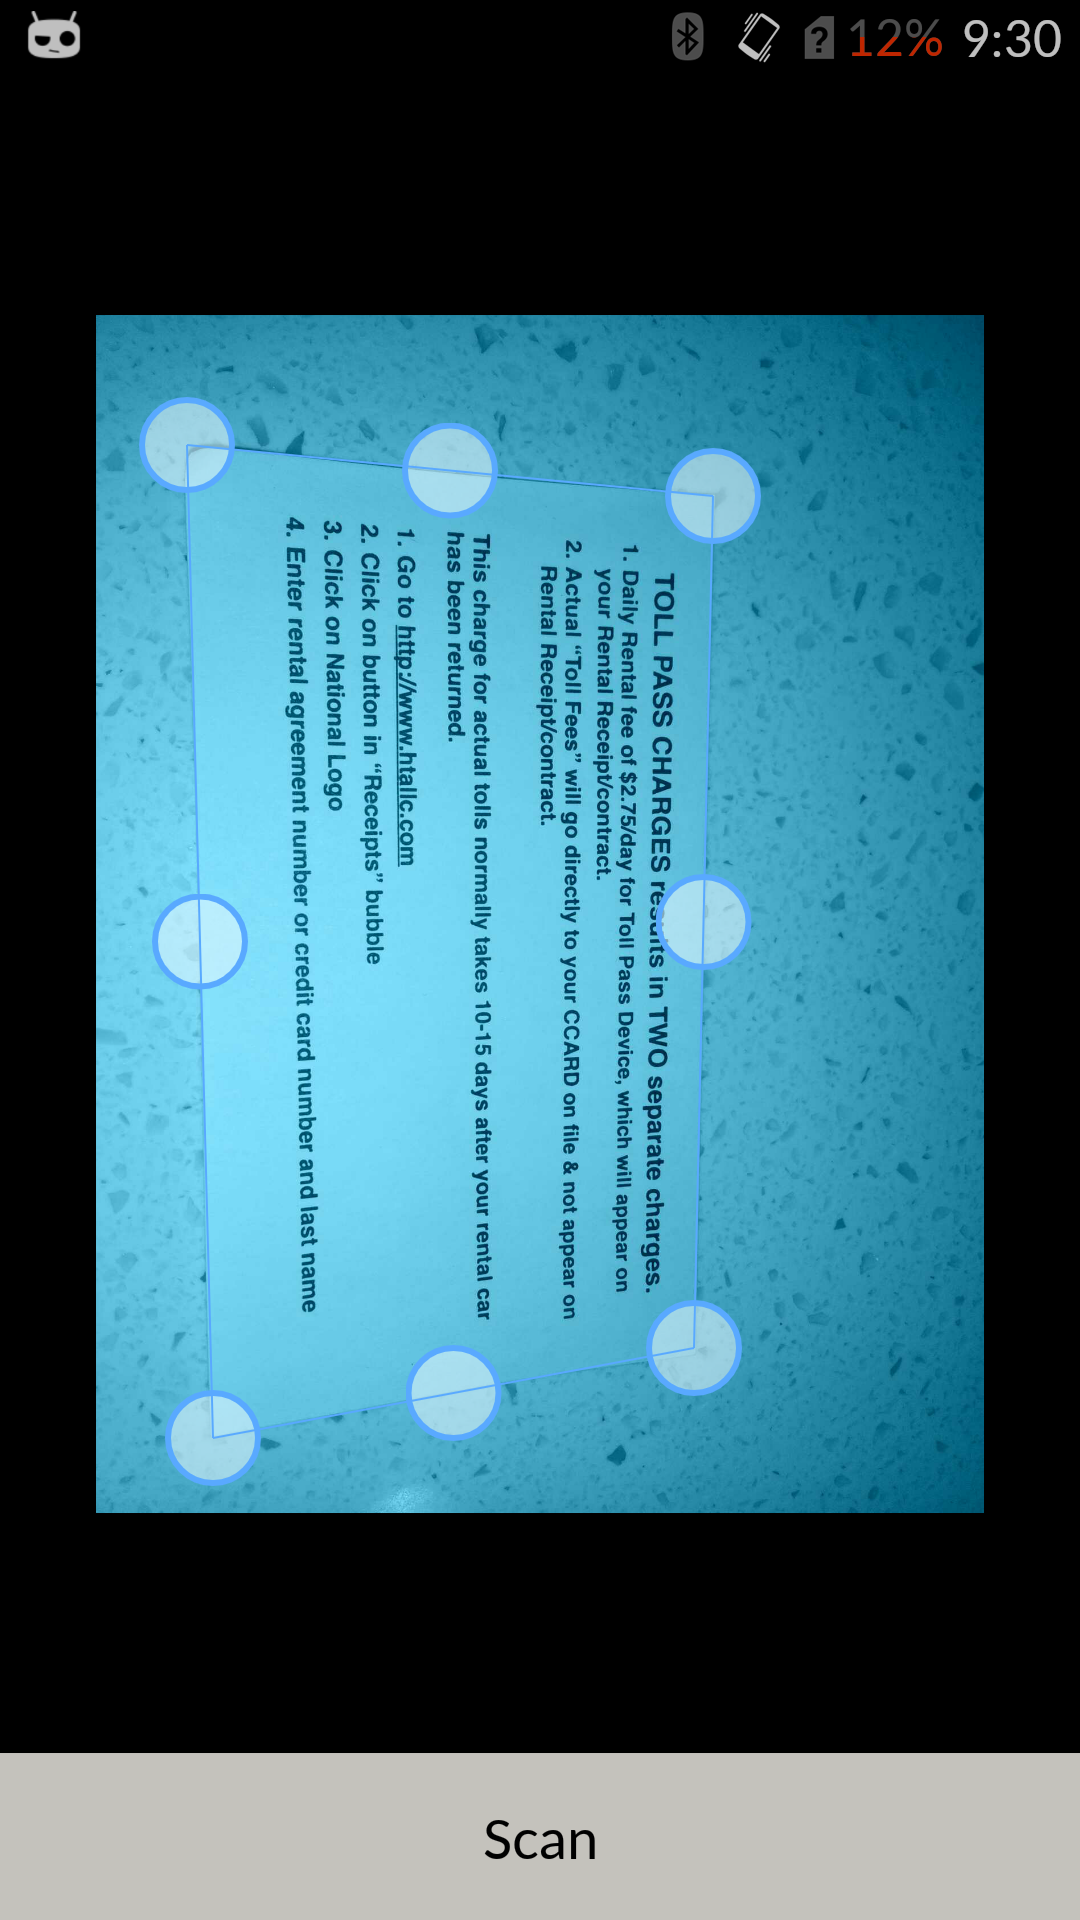
\includegraphics[width=0.3\columnwidth]{Figures/2/sc1}
		     	 	\caption{ถ่ายภาพเอกสาร}{ที่มา : https://github.com/jhansireddy/AndroidScannerDemo}
		     	 	\label{Fig:sc1}
		     	\end{figure}
		    \item ทำการปรับรูปภาพ เช่น การปรับสีรูปภาพ การปรับเป็นสีขาวดำ เป็นต้น
		      \begin{figure}[H]
		      	\centering
		      	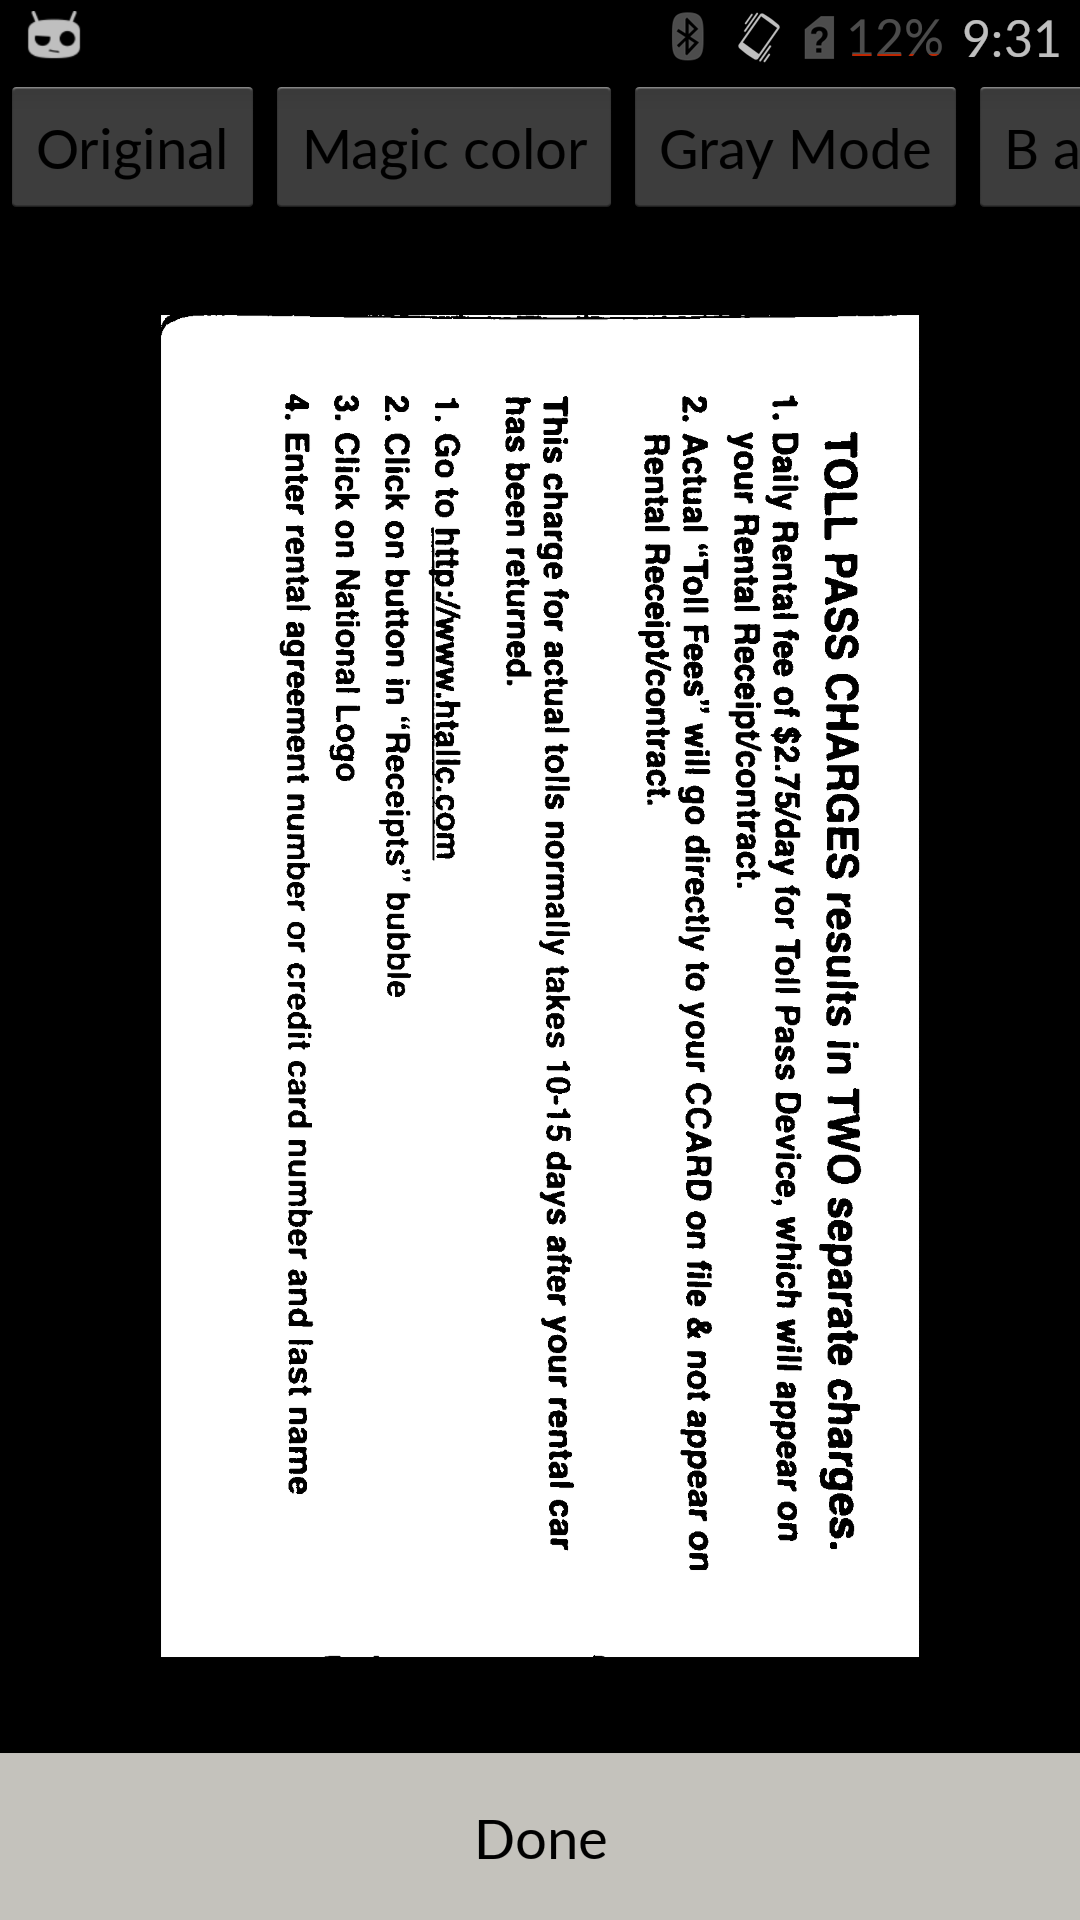
\includegraphics[width=0.3\columnwidth]{Figures/2/sc2}
		      	\caption{ปรับแต่งภาพถ่าย}{ที่มา : https://github.com/jhansireddy/AndroidScannerDemo}
		      	\label{Fig:sc2}
		      \end{figure}
		     \item ภาพที่ได้จากการประมวลผล
			     \begin{figure}[H]
			     	\centering
			     	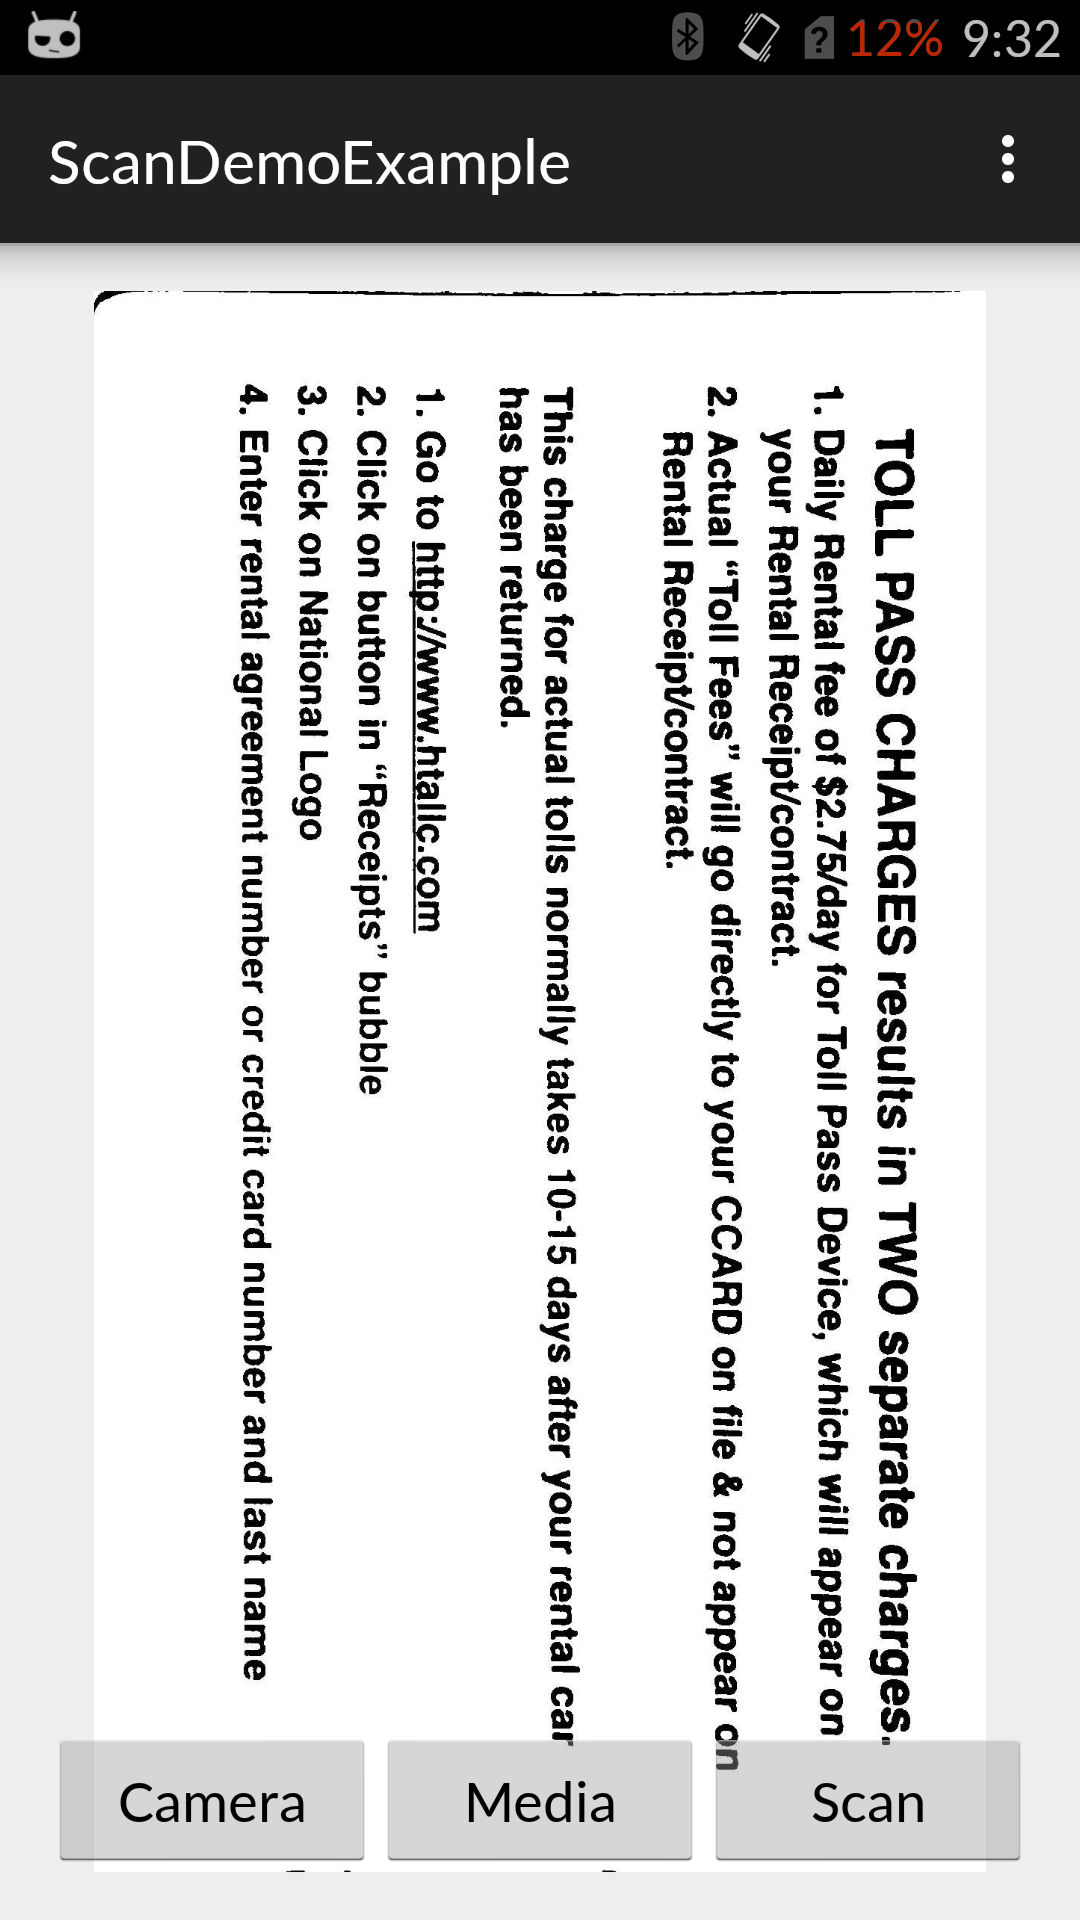
\includegraphics[width=0.3\columnwidth]{Figures/2/sc3}
			     	\caption{ผลการทำงาน}{ที่มา : https://github.com/jhansireddy/AndroidScannerDemo}
			     	\label{Fig:sc3}
			     \end{figure}
	     \end{itemize}
	     %TODO add how to implement
	     
	\section{ความรู้พื้นฐานของระบบ XX เดิม}
		 \subsection{ความเป็นมา}

      ระบบ XX เดิม มีประวัติดังนี้ 
		  
		  \subsection{วิสัยทัศน์และพันธกิจ}
		  \begin{itemize}
			  \item วิสัยทัศน์ (Vision)
			  "เป็นองค์กรหลักที่ XX"
			  
			  \item พันธกิจ (Mission)
			  \begin{enumerate}
			  	\item สนับสนุนและส่งเสริม XX 
			  	\item พัฒนาองค์กรสู่ความเป็นเลิศด้วยนวัตกรรมที่ทันสมัย โดยใช้หลักบริหารจัดการที่ดี
			  \end{enumerate}
		  \end{itemize}
	  
	  \subsection{ขั้นตอนการดำเนินการ XX}
	  \begin{itemize}
	  	\item อธิบายขั้นตอนที่ XX
	  	\item อธิบายขั้นตอนที่ XX
	  	\item อธิบายขั้นตอนที่ XX
	  \end{itemize}
	  

	\section{เอกสารและงานวิจัยที่เกี่ยวข้อง}
		  กล่าวถึงเอกสาร งานวิจัย หรือระบบงานที่คล้ายกันโดยแบ่งเป็น subsection โดยแต่ละหัวข้อให้อธิบายความสำคัญ ฟังก์ชันการทำงาน ข้อจำกัดหรือข้อแตกต่างจะระบบที่จะทำ เช่น
		 \subsection{เว็บไซต์ XX}
		 PSU Studentloan \cite{PSU} เป็นเว็บไซต์ที่ให้บริการนักศึกษากองทุนเงินให้กู้ยืมเพื่อการศึกษา มหาวิทยาลัยสงขลานครินทร์ วิทยาเขตหาดใหญ่ สามารถเข้าใช้งานได้ที่ https://studentloan.psu.ac.th/home มีฟังก์ชันการทำงานพื้นฐานอันได้แก่ การดูข่าวสารประชาสัมพันธ์  ประมวลภาพกิจกรรม ดาวน์โหลดเอกสารที่เกี่ยวข้อง เป็นต้น
			 \begin{figure}[H]
			 	\centering
			 	
\includegraphics[width=0.8\textwidth]{Figures/2/1}
			 	\caption{หน้าแรกของเว็บไซต์ PSU Studentloan}{ที่มา : https://studentloan.psu.ac.th/home}
			 	\label{Fig:Studentloan1}
			 \end{figure}
			 
		 \subsection{แอปพลิเคชัน XX}
		 eStudentloan \cite{eStudentloan} เป็นแอนดรอย์แอปพลิเคชันที่พัฒนาโดยฝ่ายกิจการนักศึกษา สถาบันเทคโนโลยีไทย-ญี่ปุ่น เพื่อให้บริการนักศึกษากองทุนเงินให้กู้ยืมเพื่อการศึกษาสถาบันเทคโนโลยีไทย-ญี่ปุ่น สามารถดาวน์โหลดเพื่อใช้งานได้ที่  https://play.google.com/store/apps/details?id=th.co.dest.anek.studentloan โดยแอปพลิเคชันมีฟังก์ชันการทำงาน คือ ติดตามข่าวสารจากหน่วยงาน 
		 \newpage
	 			\begin{figure}[H]
	 				\centering
	 				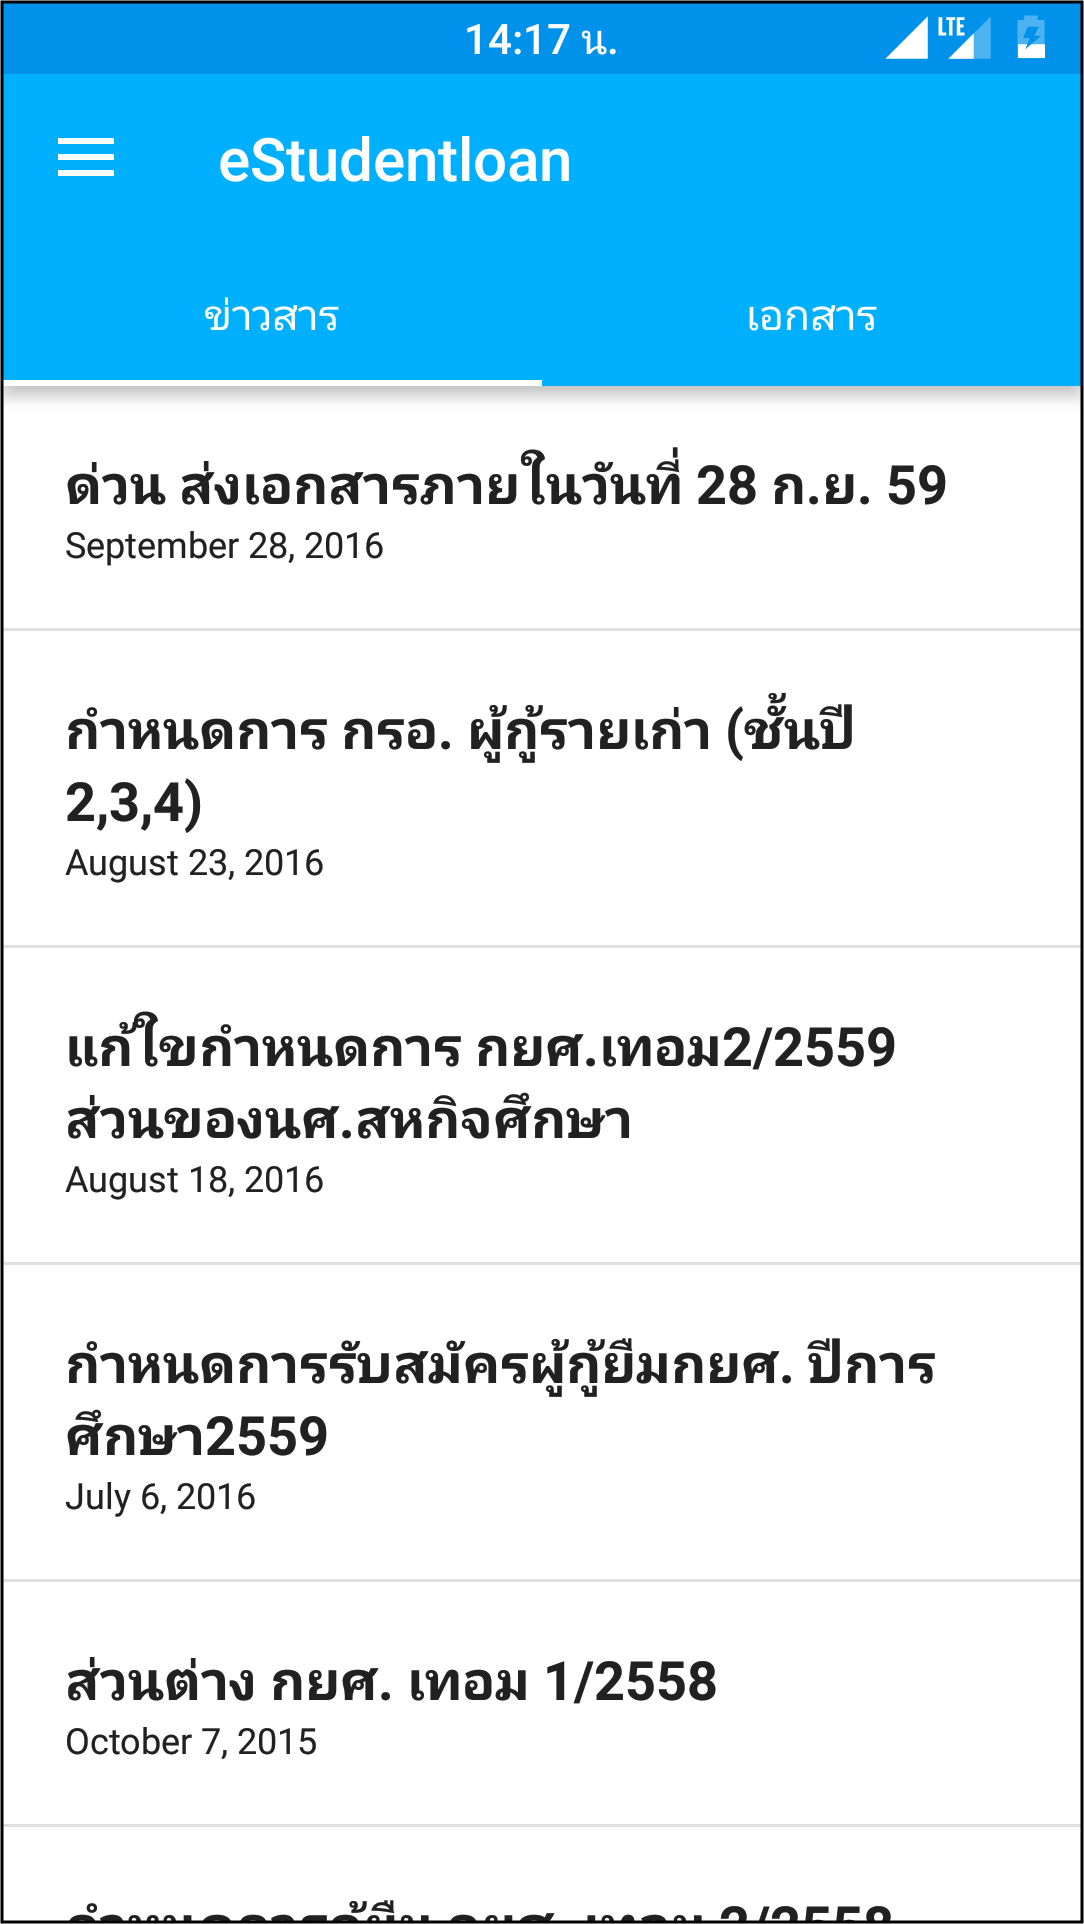
\includegraphics[width=0.45\textwidth]{Figures/2/m3}
	 				\caption{ข่าวสารจากหน่วยงาน}{ที่มา : https://play.google.com/store/apps/details?id=th.co.dest.anek.studentloan}
	 				\label{Fig:Studentloan11}
	 			\end{figure}
	
